\documentclass[a4paper, openany, 12pt]{article}

%% подключаем стандарт библиографии
\bibliographystyle{gost71u}

%% для "Abstract" в классе book
% \newenvironment{abstract}{}{}
% \usepackage{abstract}

%% подключаем преамбулу: в ней содержится подключение всех необходимых пакетов
%% Работа с русским языком
\usepackage{cmap}			 % поиск в PDF
\usepackage{mathtext} 		 % русские буквы в формулах
\usepackage[T2A]{fontenc}	 % кодировка
\usepackage[utf8]{inputenc}	 % кодировка исходного текста
\usepackage[russian]{babel}	 % локализация и переносы

%% Пакеты для работы с математикой
\usepackage{amsmath,amsfonts,amssymb,amsthm,mathtools}
\usepackage{icomma}

%% Нумерация формул (опционально)
%\mathtoolsset{showonlyrefs=true} % показывать номера только у тех формул, на которые есть \eqref{} в тексте.
%\usepackage{leqno}               % нумерация формул слева

%% Шрифты
\usepackage{mathptmx}    % Times New Roman для текста и математики
\usepackage{euscript}	 % шрифт "Евклид"
\usepackage{mathrsfs}    % красивый мат. шрифт

%% Некоторые полезные макросы для дебага (в случае недоверия авторам шаблона)
\makeatletter
\newcommand\thefontsize{The current font size is: \f@size pt} % пример: \section{\thefontsize}
\makeatother

%% Настройка размеров шрифтов
\makeatletter
\setlength{\headheight}{28pt}
%% TODO: мне не удалось разобраться, как грамотно подбирать второе число в
%% \@setfontsize\*, но ряд экспериментов показывает, что "10" выравнивает текст весьма прилично :)
\renewcommand\Huge{\@setfontsize\Huge{14pt}{10}}
\renewcommand\huge{\@setfontsize\huge{14pt}{10}}
\renewcommand\Large{\@setfontsize\Large{14pt}{10}}
\renewcommand\large{\@setfontsize\large{12pt}{10}}
\makeatother

%% Поля (геометрия страницы)
\usepackage[left=3cm,right=1.5cm,top=2cm,bottom=2cm,bindingoffset=0cm]{geometry}

%% Русские списки
\usepackage{enumitem}
\makeatletter
\AddEnumerateCounter{\asbuk}{\russian@alph}{щ}
\makeatother

%% Работа с картинками
\usepackage{caption} % пакет для подписей к рисункам, в частности, для работы caption*
\captionsetup{justification=centering} % центрирование подписей к картинкам
\usepackage{graphicx}                  % вставки рисунков
\graphicspath{{images/}{images2/}}     % папки с картинками
\setlength\fboxsep{3pt}                % отступ рамки \fbox{} от рисунка
\setlength\fboxrule{1pt}               % толщина линий рамки \fbox{}
\usepackage{wrapfig}                   % обтекание рисунков и таблиц текстом

%% Работа с таблицами
\usepackage{array,tabularx,tabulary,booktabs} % дополнительная работа с таблицами
\usepackage{longtable}                        % длинные таблицы
\usepackage{multirow}                         % слияние строк и столбцов в таблице
\usepackage{makecell}                         % создание ячеек с многими строчками текста
\usepackage{hhline}                           % позволяет разрывать горизонтальные линии в таблицах

%% Красная строка
\setlength{\parindent}{1.25cm}

%% Интервалы
\linespread{1.3}

%% TikZ
\usepackage{tikz}
\usetikzlibrary{graphs,graphs.standard}

%% Верхний колонтитул
\usepackage{fancyhdr}
\pagestyle{fancy}

%% Перенос знаков в формулах (по Львовскому)
\newcommand*{\hm}[1]{#1\nobreak\discretionary{}{\hbox{$\mathsurround=0pt #1$}}{}}

%% Дополнительно
\usepackage{float}   % добавляет возможность работы с командой [H] которая улучшает расположение на странице
\usepackage{gensymb} % красивые градусы
\usepackage{listings} % пакет для листингов с кодом
\lstset{              % настройки для лисингов с кодом
basicstyle=\small\ttfamily,
columns=flexible,
breaklines=true
}

% Hyperref (для ссылок внутри  pdf)
\usepackage[unicode, pdftex]{hyperref}

% Отступ перед первым абзацем в каждом разделе
\usepackage{indentfirst}

%% Теоремные окружения (amsthm)
\newtheoremstyle{spacedplain}
    {14pt}   % отступ перед окружением
    {14pt}   % отступ после окружения
    {\itshape}
    {}
    {\bfseries}
    {.}
    {.5em}
    {}
\newtheoremstyle{spaceddefinition}
    {14pt}
    {14pt}
    {}
    {}
    {\bfseries}
    {.}
    {.5em}
    {}
\theoremstyle{spacedplain}
\newtheorem{theorem}{Теорема}[section]
\newtheorem{lemma}[theorem]{Лемма}
\newtheorem{corollary}[theorem]{Следствие}
\newtheorem{proposition}[theorem]{Предложение}
\theoremstyle{spaceddefinition}
\newtheorem{definition}[theorem]{Определение}
\newtheorem{remark}[theorem]{Замечание}


\begin{document}
    %% титульник
    \begin{center}
    %% *название института*
    \large\textbf{Министерство науки и высшего образования Российской Федерации\\
    Московский физико-технический институт (государственный
    университет)} \\
    \vspace{1cm}

    %% *факультет/физтех-школа*
    Физтех-школа прикладной математики и информатики \\

    %% *название базовой кафедры и лаборатории*
    %% в случае ненадобности можно удалить
    Кафедра интеллектуального анализа данных \\
    Вычислительный центр
им. А.А. Дородницына
Российской академии наук
Федерального исследовательского центра
«Информатика и управление»
Российской академии наук
 \\

    \vspace{3em}

    Выпускная квалификационная работа бакалавра
\end{center}

\begin{center}
    \vspace{\fill}
    %% *название вашей работы*
    \LARGE{% Единое место для указания названия работы
Алгоритм распознавания скрытых петель обратной связи в рекомендательных системах}

    \vspace{\fill}
\end{center}


\begin{flushright}
    \textbf{Автор:} \\
    Студент Б05-203 группы \\
    Дементьев Сергей Андреевич \\
    \vspace{2em}
    \textbf{Научный руководитель:} \\
    к.ф.-м.н. \\
    Хританков Антон Сергеевич \\

\end{flushright}

\vspace{7em}

\begin{center}
    %% *лого*
    
\includegraphics[width=100 pt]{MIPT_logo.jpg}\\
    Москва \the\year{}
\end{center}

%% выключаем отображение номера для этой страницы (титульник)
\thispagestyle{empty}

    \newpage

    \setcounter{page}{2}
    \fancyfoot[c]{\thepage}
    %% *надпись над верхним колонтитулом*
    %% в случае ненадобности можно удалить
    \fancyhead[L]{% Единое место для указания названия работы
Алгоритм распознавания скрытых петель обратной связи в рекомендательных системах}
    \fancyhead[R]{}

    %% аннотация
    \begin{abstract}

    \begin{center}
        \large{% Единое место для указания названия работы
Алгоритм распознавания скрытых петель обратной связи в рекомендательных системах} \\
    \large\textit{Деметьев Сергей Андреевич} \\[1 cm]

    Краткое описание задачи и основных результатов, мотивирующее прочитать весь текст.

    \vfill

    \textbf{Abstract} \\[1 cm]

    Research and development of machine learning methods
    \end{center}

\end{abstract}

    \newpage

    %% содержание
    \tableofcontents{}
    \newpage

    % \fontsize{14}{16}\selectfont
    \section{Введение}
\label{sec:Chapter0} \index{Chapter0}

% -----------------------------------------------------------------------
% 1. АКТУАЛЬНОСТЬ И КОНТЕКСТ
% -----------------------------------------------------------------------

Современные промышленные рекомендательные системы работают в условиях
непрерывной обратной связи: модель формирует выдачу, пользователь реагирует
на неё, журналы взаимодействий поступают в обучающую выборку следующей
итерации дообучения. Такой режим эксплуатации принципиально отличается от
стандартного предположения машинного обучения о независимой и одинаково
распределённой выборке (i.i.d.): распределение обучающих данных на каждом
шаге зависит от параметров модели на предыдущем шаге. Это явление принято
называть \textit{скрытой петлёй обратной связи} (hidden feedback loop).

Проблема hidden feedback loops в системах машинного обучения изучается
как в контексте общей теории repeated learning, так и применительно
к конкретным классам задач: ранжирование, фильтрация контента,
персонализация новостных лент. В рекомендательных системах эта петля
замкнута особенно тесно: пользователь видит только то, что система
рекомендует, а система обучается только на том, что пользователь увидел и
на что отреагировал. Следовательно, области пространства объектов,
недоступные пользователю в момент времени $t$, выпадают из обучающей
выборки момента $t{+}1$. Накопленный эффект многократного повторения этого
цикла может привести к систематическому сужению выдачи и, в пределе, к
формированию так называемых \textit{эхо-камер}~--- режима, при котором
разные кластеры пользователей получают диверсифицированные, но внутренне
однородные рекомендации без пересечения с контентом других кластеров.

Геометрическая интерпретация этого явления связана с изменением структуры
пользовательских предпочтений в процессе repeated learning. Если
рассматривать состояние системы как распределение вероятностей в
пространстве пользователей, то каждая итерация переобучения действует как
оператор, трансформирующий это распределение. При определённых условиях
такой оператор оказывается сжимающим: внутрикластерное разнообразие
убывает, а межкластерные границы становятся резче. Анализ условий, при
которых это сжатие неизбежно, и является центральным предметом настоящей
работы.

% -----------------------------------------------------------------------
% 2. ОБЪЕКТ И ПРЕДМЕТ ИССЛЕДОВАНИЯ
% -----------------------------------------------------------------------

\textbf{Объектом исследования} является рекомендательная система,
функционирующая в режиме онлайн-переобучения с обратной связью по
пользовательским реакциям.

\textbf{Предметом исследования} служит геометрия распределения
рекомендаций в пространстве пользователей в условиях repeated learning:
в частности, условия затухания внутрикластерной дисперсии выдачи и
возникновения эхо-камерного режима.

% -----------------------------------------------------------------------
% 3. ЦЕЛЬ И ЗАДАЧИ
% -----------------------------------------------------------------------

\textbf{Цель работы}~--- построить теоретическую модель, описывающую
долгосрочную динамику персонализации в рекомендательной системе с обратной
связью, и установить условия, при которых эта динамика приводит к
деградации микроперсонализации.

Для достижения поставленной цели необходимо решить следующие задачи:
\begin{enumerate}
    \item Формализовать рекомендательную систему с повторяющимся
          переобучением как дискретную динамическую систему на пространстве
          распределений пользователей и объектов.
    \item Ввести кластерную структуру аудитории и получить локальную
          линеаризацию оператора переобучения вблизи стационарного
          распределения.
    \item Исследовать спектральные свойства эффективного оператора
          переобучения и установить условия его сжимающего действия на
          внутрикластерные ковариации.
    \item Доказать теорему о коллапсе персонализации: при выполнении условий
          сжатия распределение рекомендаций сходится к $K$-модальной
          комбинации дельта-мер.
    \item Верифицировать теоретические выводы численно на синтетических и
          реальных данных, измерив динамику внутрикластерного разнообразия
          при различных режимах переобучения.
    \item Проанализировать влияние управляющих параметров~--- уровня
          exploration и силы регуляризации~--- на предельный режим системы
          и установить достаточные условия сохранения ненулевого разнообразия.
\end{enumerate}

% -----------------------------------------------------------------------
% 4. МЕТОДЫ ИССЛЕДОВАНИЯ
% -----------------------------------------------------------------------

В работе используются методы теории динамических систем на пространствах
мер (операторный подход, теория сжимающих отображений), линейной алгебры
и спектральной теории (анализ спектрального радиуса, сингулярное
разложение), теории вероятностей (ковариационная динамика, слабая
сходимость мер), а также вычислительные методы: моделирование repeated
recommendation loop на синтетических данных и датасете MovieLens.

% -----------------------------------------------------------------------
% 5. НАУЧНАЯ НОВИЗНА И ПРАКТИЧЕСКАЯ ЗНАЧИМОСТЬ
% -----------------------------------------------------------------------

\textbf{Научная новизна} работы состоит в следующем. Во-первых, предложена
кластерная динамическая модель рекомендательной системы, явно учитывающая
зависимость обучающих данных от политики рекомендаций. Во-вторых, получены
спектральные условия, при которых оператор переобучения является сжимающим
по внутрикластерным ковариациям. В-третьих, доказана теорема о сходимости
распределения рекомендаций к $K$-модальной эхо-камере и установлена
зависимость скорости этой сходимости от параметров модели.

\textbf{Практическая значимость} определяется тем, что полученные
теоретические условия допускают непосредственную проверку по наблюдаемым
статистикам системы и могут служить основой для разработки метрик
мониторинга риска коллапса персонализации в промышленных рекомендательных
системах.

% -----------------------------------------------------------------------
% 6. СТРУКТУРА РАБОТЫ
% -----------------------------------------------------------------------

Работа организована следующим образом. В~главе~\ref{sec:Chapter1}
рекомендательная система формализуется как repeated learning process и
ставится основной исследовательский вопрос. Глава~\ref{sec:Chapter2}
посвящена построению математической модели: вводятся кластерная структура
аудитории, локальная линеаризация рекомендательной политики и ковариационная
динамика выдачи. В~главе~\ref{sec:Chapter3} формулируются и доказываются
основные теоремы~--- о спектральном сжатии и коллапсе персонализации.
Глава~\ref{sec:Chapter4} описывает вычислительный эксперимент и анализирует
соответствие численных результатов теоретическим предсказаниям.
Глава~\ref{sec:Chapter5} рассматривает управляемую версию модели и анализирует
условия предотвращения коллапса через exploration и регуляризацию. В
заключении (глава~\ref{sec:Chapter6}) формулируются итоги работы и
направления дальнейших исследований.
 %% Введение
    \newpage
    \section{Постановка задачи}
\label{sec:Chapter1} \index{Chapter1}

% -----------------------------------------------------------------------
% 1.1 РЕКОМЕНДАТЕЛЬНАЯ СИСТЕМА КАК REPEATED LEARNING PROCESS
% -----------------------------------------------------------------------

\subsection{Рекомендательная система как процесс с обратной связью}
\label{subsec:rl_process}

Зафиксируем конечное множество пользователей $\mathcal{U}$ и конечное
множество объектов (айтемов) $\mathcal{I}$, $|\mathcal{U}|=N$,
$|\mathcal{I}|=M$. На каждом дискретном шаге времени $t=0,1,2,\ldots$
рекомендательная система выполняет три операции:

\begin{enumerate}
    \item \textbf{Рекомендация.} Для каждого пользователя $u \in \mathcal{U}$
          система выбирает подмножество объектов $S^{(t)}_u \subseteq
          \mathcal{I}$ для показа в соответствии с текущей политикой
          $\pi^{(t)}$.

    \item \textbf{Пользовательский отклик.} Пользователь $u$ взаимодействует
          с показанными объектами; формируется множество наблюдений
          $\mathcal{D}^{(t)}_u = \{(u, i, r^{(t)}_{ui}) : i \in S^{(t)}_u\}$,
          где $r^{(t)}_{ui} \in \mathbb{R}$ фиксирует реакцию (оценку,
          клик, время просмотра и т.\,д.).

    \item \textbf{Переобучение.} Параметры модели обновляются по накопленным
          данным $\mathcal{D}^{(t)} = \bigcup_{u} \mathcal{D}^{(t)}_u$, порождая
          политику $\pi^{(t+1)}$.
\end{enumerate}

Принципиальное отличие этого цикла от стандартной схемы обучения с учителем
состоит в том, что $\mathcal{D}^{(t)}$ есть функционал от политики $\pi^{(t)}$:
объекты, не попавшие в выдачу $S^{(t)}_u$, не порождают обучающих примеров
для шага $t{+}1$. Следовательно, задача оценки модели по наблюдаемым данным
принципиально смещена~--- это явление называется \textit{selection bias},
индуцированным самой рекомендательной системой.

\subsection{Пространство состояний и оператор переобучения}
\label{subsec:state_space}

Для описания долгосрочной динамики введём пространство состояний.
Обозначим через $\mathcal{P}(\mathcal{U})$ множество вероятностных мер
на $\mathcal{U}$; аналогично $\mathcal{P}(\mathcal{I})$~--- вероятностные
меры на $\mathcal{I}$. Состояние системы в момент $t$ задаётся парой
$(\mu^{(t)}, \nu^{(t)}) \in \mathcal{P}(\mathcal{U}) \times
\mathcal{P}(\mathcal{I})$, где $\mu^{(t)}$ описывает активность
пользователей, а $\nu^{(t)}$~--- распределение популярности объектов
в обучающей выборке.

\begin{definition}[Оператор переобучения]
\label{def:retraining_op}
\textit{Оператором переобучения} называется отображение
\[
    \mathcal{F} \colon \mathcal{P}(\mathcal{U}) \times
    \mathcal{P}(\mathcal{I}) \;\longrightarrow\;
    \Pi,
\]
сопоставляющее распределению данных $(\mu, \nu)$ политику рекомендаций
$\pi = \mathcal{F}(\mu, \nu)$, получаемую минимизацией функционала потерь
по обучающей выборке с распределением $(\mu, \nu)$.
\end{definition}

Совместно с оператором пользовательского отклика
$\mathcal{G} \colon \Pi \to \mathcal{P}(\mathcal{U}) \times \mathcal{P}(\mathcal{I})$
(преобразующим политику в распределение наблюдаемых реакций) оператор
переобучения задаёт дискретную динамическую систему
\[
    (\mu^{(t+1)},\, \nu^{(t+1)}) \;=\; \mathcal{G}\!\bigl(\mathcal{F}(\mu^{(t)},\, \nu^{(t)})\bigr).
\]

% -----------------------------------------------------------------------
% 1.2 КЛАСТЕРНАЯ СТРУКТУРА И ЛОКАЛЬНОЕ РАЗНООБРАЗИЕ
% -----------------------------------------------------------------------

\subsection{Кластерная структура аудитории}
\label{subsec:cluster_structure}

Предполагается, что пользователи образуют $K$ кластеров
$\mathcal{C}_1, \ldots, \mathcal{C}_K$ (например, по сегментам вкусовых
предпочтений). Пусть $\mu_k^{(t)} = \mu^{(t)}(\mathcal{C}_k)$~--- доля
кластера $k$ в момент $t$, и пусть $\overline{x}_k^{(t)}$~---
центроид (вектор средних предпочтений) кластера $k$, а
$\Sigma_k^{(t)}$~--- ковариационная матрица пользовательских
предпочтений внутри кластера $k$.

\begin{definition}[Внутрикластерное разнообразие]
\label{def:diversity}
\textit{Внутрикластерным разнообразием} в момент $t$ называется
суммарный след ковариационных матриц:
\[
    D^{(t)} \;=\; \sum_{k=1}^{K} \mu_k^{(t)} \,\operatorname{tr}\!\bigl(\Sigma_k^{(t)}\bigr).
\]
\end{definition}

\begin{definition}[Эхо-камера]
\label{def:echo_chamber}
Говорим, что система \textit{достигла режима эхо-камеры} к моменту $T$,
если для каждого кластера $k$ распределение рекомендаций в $\mathcal{C}_k$
сосредоточено в $\varepsilon$-окрестности единственного объекта
$i^*_k \in \mathcal{I}$:
\[
    \pi^{(T)}\bigl(S^{(T)}_u \ni i \bigr) < \varepsilon
    \quad \forall\, u \in \mathcal{C}_k,\; i \neq i^*_k.
\]
В пределе $\varepsilon \to 0$ это означает сходимость распределения
рекомендаций к $K$-модальной сумме дельта-мер:
\[
    \pi^{(\infty)} \;\xrightarrow{w}\; \sum_{k=1}^{K} \mu_k \,\delta_{i^*_k}.
\]
\end{definition}

% -----------------------------------------------------------------------
% 1.3 ФОРМУЛИРОВКА ИССЛЕДОВАТЕЛЬСКОГО ВОПРОСА
% -----------------------------------------------------------------------

\subsection{Исследовательский вопрос}
\label{subsec:research_question}

Таким образом, основной исследовательский вопрос формулируется следующим
образом.

\begin{quote}
\textit{При каких условиях на операторы $\mathcal{F}$ и $\mathcal{G}$,
кластерную структуру $\{\mathcal{C}_k\}$ и начальное состояние
$(\mu^{(0)}, \nu^{(0)})$ динамика системы приводит к обращению
внутрикластерного разнообразия $D^{(t)} \to 0$ при $t \to \infty$,
то есть к режиму $K$-модальной эхо-камеры?}
\end{quote}

Дополнительный вопрос касается управляемости: при каких значениях
параметра exploration $\alpha \in [0,1]$ и регуляризационного
коэффициента $\lambda > 0$ разнообразие $D^{(t)}$ сохраняется
ненулевым при $t \to \infty$?

Ответы на эти вопросы получены в главах~\ref{sec:Chapter2}
и~\ref{sec:Chapter3}.
 %% Постановка задачи
    \newpage
    \section{Математическая модель рекомендательной системы с обратной связью}
\label{sec:Chapter2} \index{Chapter2}

% -----------------------------------------------------------------------
% 2.1 ЛОКАЛЬНАЯ ЛИНЕАРИЗАЦИЯ РЕКОМЕНДАТЕЛЬНОЙ ПОЛИТИКИ
% -----------------------------------------------------------------------

\subsection{Локальная линеаризация рекомендательной политики}
\label{subsec:local_linearization}

Пусть $\bar{w}$~--- параметры модели в стационарной точке и пусть
$f(u, i; w) \in \mathbb{R}$~--- скоринговая функция (оценка релевантности
объекта $i$ пользователю $u$ при параметрах $w$). Разложим $f$ по
параметрам вблизи $\bar{w}$:
\[
    f(u, i; w) \;\approx\; f(u, i; \bar{w}) \;+\;
    \bigl\langle \nabla_w f(u, i; \bar{w}),\, w - \bar{w} \bigr\rangle.
\]

Обозначим через $J_{ui} = \nabla_w f(u, i; \bar{w}) \in \mathbb{R}^p$
вектор-градиент скоринговой функции по параметрам в стационарной точке.
Тогда линеаризованная рекомендательная политика задаётся матрицей Якоби
$\mathbf{J} \in \mathbb{R}^{NM \times p}$, строки которой~--- это
$J_{ui}$ для всех пар $(u, i)$.

\begin{definition}[Локальный Якобиан рекомендательной политики]
\label{def:local_jacobian}
\textit{Локальным Якобианом} политики в кластере $k$ называется матрица
\[
    \mathbf{J}_k \;=\;
    \frac{1}{|\mathcal{C}_k||\mathcal{I}|}
    \sum_{u \in \mathcal{C}_k} \sum_{i \in \mathcal{I}}
    J_{ui} J_{ui}^\top \;\in\; \mathbb{R}^{p \times p},
\]
то есть усреднённая матрица внешних произведений градиентов по парам
пользователь-объект внутри кластера.
\end{definition}

Ключевое наблюдение: $\mathbf{J}_k$ отвечает за то, насколько
чувствительна рекомендательная политика к индивидуальным различиям
пользователей внутри кластера $k$. Если $\operatorname{rank}(\mathbf{J}_k)$
мало или $\mathbf{J}_k$ имеет маленький спектральный радиус,
политика практически не различает пользователей внутри кластера.

% -----------------------------------------------------------------------
% 2.2 КОВАРИАЦИОННАЯ ДИНАМИКА ВЫДАЧИ
% -----------------------------------------------------------------------

\subsection{Ковариационная динамика выдачи}
\label{subsec:covariance_dynamics}

Рассмотрим, как эволюционирует ковариационная матрица
$\Sigma_k^{(t)}$ под действием одного шага переобучения.

Пусть $\delta w^{(t)} = w^{(t+1)} - w^{(t)}$~--- изменение параметров
модели на шаге $t$. В линейном приближении это изменение пропорционально
стохастическому градиенту функционала потерь по наблюдаемым данным.
Для выдачи пользователя $u$ получаем:
\[
    \delta\hat{r}^{(t)}_u \;=\; \mathbf{J}^\top_u \,\delta w^{(t)},
\]
где $\mathbf{J}_u \in \mathbb{R}^{p \times M}$~--- матрица градиентов
по объектам для пользователя $u$.

\begin{proposition}[Рекуррентность ковариаций]
\label{prop:covariance_recursion}
В линейном приближении ковариационная матрица выдачи в кластере $k$
удовлетворяет рекуррентному соотношению:
\[
    \Sigma_k^{(t+1)} \;=\;
    \mathbf{A}_k\, \Sigma_k^{(t)}\, \mathbf{A}_k^\top
    \;+\; \mathbf{B}_k,
\]
где $\mathbf{A}_k$~--- \textup{эффективный оператор переобучения} для
кластера $k$, а $\mathbf{B}_k$~--- матрица, описывающая внешний шум
и exploration. Явные выражения для $\mathbf{A}_k$ и $\mathbf{B}_k$
выведены в приложении~\textup{A}.
\end{proposition}

Структура предложения~\ref{prop:covariance_recursion}~--- это матричное
уравнение дискретного Ляпунова. Долгосрочное поведение $\Sigma_k^{(t)}$
определяется спектральным радиусом $\rho(\mathbf{A}_k)$: если
$\rho(\mathbf{A}_k) < 1$, ковариации затухают; если $\rho(\mathbf{A}_k)
\geq 1$ при $\mathbf{B}_k = 0$~--- растут или стабилизируются.

% -----------------------------------------------------------------------
% 2.3 ЭФФЕКТИВНАЯ ДИНАМИКА ПЕРЕОБУЧЕНИЯ
% -----------------------------------------------------------------------

\subsection{Эффективная динамика переобучения}
\label{subsec:effective_retraining}

Связь между локальным Якобианом $\mathbf{J}_k$ и эффективным
оператором $\mathbf{A}_k$ устанавливается через матрицу Хессе
функционала потерь $\mathbf{H}^{(t)}$. При обучении методом градиентного
спуска с шагом $\eta$ получаем приближение:
\[
    \mathbf{A}_k \;\approx\; \mathbf{I} \;-\;
    \eta\, \mathbf{H}^{(t)}\big|_{\mathcal{C}_k}.
\]

Таким образом, спектральный радиус $\rho(\mathbf{A}_k)$ определяется
минимальными собственными значениями Хессе функционала потерь на
данных кластера $k$. Если Хессе вырожден или имеет малые собственные
значения (что типично для переобученных моделей), $\rho(\mathbf{A}_k)$
оказывается близким к $1$ или превышает $1$, и ковариации не затухают.

% -----------------------------------------------------------------------
% 2.4 ЗАМКНУТАЯ СИСТЕМА: ДИНАМИКА ПОЛЬЗОВАТЕЛЕЙ И EXPLORATION
% -----------------------------------------------------------------------

\subsection{Замкнутая система: динамика пользователей и exploration}
\label{subsec:full_system}

Чтобы модель была замкнутой и допускала анализ предельных режимов,
необходимо учесть два дополнительных элемента.

\textbf{Динамика пользователей.} Предполагается, что вектор предпочтений
пользователя $u$ медленно дрейфует под влиянием получаемых рекомендаций:
\[
    x_u^{(t+1)} \;=\; (1-\beta)\, x_u^{(t)} \;+\; \beta\,
    \operatorname{softmax}_{i}\!\bigl(f(u,i;w^{(t)})\bigr),
\]
где $\beta \in [0,1]$~--- коэффициент влияния рекомендаций на предпочтения.
При $\beta = 0$ пользователи статичны; при $\beta > 0$ их предпочтения
смещаются в сторону рекомендованных объектов.

\textbf{Параметр exploration.} В политику рекомендаций вводится
смешивание с равномерным распределением по объектам:
\[
    \pi^{(t)}_\alpha(i \mid u) \;=\;
    (1 - \alpha)\,\pi^{(t)}(i \mid u) \;+\; \frac{\alpha}{M},
    \quad \alpha \in [0,1].
\]
Параметр $\alpha$ контролирует степень исследования пространства объектов;
при $\alpha = 0$ система работает в чисто эксплуатационном режиме.

Полная замкнутая система описывается совместной эволюцией параметров
$w^{(t)}$, пользовательских предпочтений $\{x_u^{(t)}\}$ и политики
$\pi^{(t)}_\alpha$. Её анализ~--- в частности, условия сходимости к
стационарному распределению и существование предельных режимов с
ненулевым разнообразием~--- проводится в главе~\ref{sec:Chapter3}.
 %% Математическая модель
    \newpage
    \section{Теоремы о спектральном сжатии и коллапсе персонализации}
\label{sec:Chapter3} \index{Chapter3}

% -----------------------------------------------------------------------
% 3.1 КОРРЕКТНОСТЬ ЛОКАЛЬНОЙ ДИНАМИКИ
% -----------------------------------------------------------------------

\subsection{Корректность локальной динамики}
\label{subsec:well_posedness}

Прежде чем формулировать результаты о сходимости, установим корректность
построенной модели: существование стационарных точек и применимость
линеаризации в их окрестностях.

\begin{proposition}[Существование стационарной точки]
\label{prop:fixed_point}
При выполнении условий \textup{(A1)--(A3)} (компактность пространств
$\mathcal{U}$, $\mathcal{I}$, равномерная сходимость эмпирического
функционала) отображение $\Phi = \mathcal{G} \circ \mathcal{F}$
допускает по крайней мере одну неподвижную точку
$(\bar\mu, \bar\nu) \in \mathcal{P}(\mathcal{U}) \times
\mathcal{P}(\mathcal{I})$.
\end{proposition}

\textit{Доказательство.} Применение теоремы Какутани к компактному
выпуклому пространству мер и полунепрерывному снизу оператору $\Phi$.
\hfill$\square$

Содержательно предложение~\ref{prop:fixed_point} означает, что
рекомендательная система всегда достигает некоторого режима
«самосогласованности»: существует политика и соответствующее
распределение данных, при которых переобучение не меняет политику.
Вопрос в том, является ли этот режим разнообразным или деградировавшим.

% -----------------------------------------------------------------------
% 3.2 СПЕКТРАЛЬНОЕ СЖАТИЕ ОПЕРАТОРА ПЕРЕОБУЧЕНИЯ
% -----------------------------------------------------------------------

\subsection{Спектральное сжатие оператора переобучения}
\label{subsec:spectral_contraction}

Центральный технический результат работы~--- теорема о спектральном
сжатии.

\begin{theorem}[Спектральное сжатие]
\label{thm:spectral_contraction}
Пусть выполнены условия \textup{(A1)--(A5)}. Пусть шаг градиентного
спуска $\eta$ удовлетворяет $\eta < 2/\lambda_{\max}(\mathbf{H})$,
и пусть параметр exploration равен нулю ($\alpha = 0$). Тогда для
эффективного оператора переобучения кластера $k$ выполнено:
\[
    \rho(\mathbf{A}_k) \;\leq\;
    1 - \eta\,\lambda_{\min}^+(\mathbf{H}\big|_{\mathcal{C}_k}),
\]
где $\lambda_{\min}^+$ обозначает минимальное положительное собственное
значение.
\end{theorem}

\textit{Доказательство.} Следует из явного представления
$\mathbf{A}_k \approx \mathbf{I} - \eta\,\mathbf{H}\big|_{\mathcal{C}_k}$
и оценки нормы возмущения по теореме Вейля. Подробный вывод~---
в приложении~A. \hfill$\square$

Если кластерный Хессе не вырожден (что выполнено, например, при
$L_2$-регуляризации с коэффициентом $\lambda > 0$), то
$\lambda_{\min}^+(\mathbf{H}\big|_{\mathcal{C}_k}) \geq \lambda$,
и $\rho(\mathbf{A}_k) \leq 1 - \eta\lambda < 1$. Это означает
экспоненциальное затухание ковариаций.

% -----------------------------------------------------------------------
% 3.3 ЗАТУХАНИЕ ЛОКАЛЬНОГО ЯКОБИАНА
% -----------------------------------------------------------------------

\subsection{Затухание локального Якобиана и исчезновение разнообразия}
\label{subsec:jacobian_decay}

Из теоремы~\ref{thm:spectral_contraction} немедленно следует результат
об убывании внутрикластерного разнообразия.

\begin{corollary}[Затухание разнообразия]
\label{cor:diversity_decay}
При условиях теоремы~\ref{thm:spectral_contraction} и $\alpha = 0$
внутрикластерное разнообразие удовлетворяет:
\[
    D^{(t)} \;\leq\; D^{(0)}\,
    \bigl(1 - \eta\,\lambda_{\min}^+\bigr)^{2t}
    \;\xrightarrow[t \to \infty]{}\; 0.
\]
\end{corollary}

Следствие~\ref{cor:diversity_decay} означает, что даже если на момент
$t=0$ пользователи внутри каждого кластера имеют разнообразные
предпочтения (ненулевая $\Sigma_k^{(0)}$), повторяющееся переобучение
стирает это разнообразие экспоненциально быстро.

% -----------------------------------------------------------------------
% 3.4 ТЕОРЕМА О КОЛЛАПСЕ ПЕРСОНАЛИЗАЦИИ (ЭХО-КАМЕРА)
% -----------------------------------------------------------------------

\subsection{Теорема о коллапсе персонализации}
\label{subsec:collapse_theorem}

Главный теоретический результат работы.

\begin{theorem}[Коллапс персонализации]
\label{thm:personalization_collapse}
Пусть выполнены условия теоремы~\ref{thm:spectral_contraction},
и пусть дополнительно функция отклика $\mathcal{G}$ непрерывна по
распределению рекомендаций в слабой топологии. Тогда при $\alpha = 0$
и любом начальном состоянии $(\mu^{(0)}, \nu^{(0)})$ распределение
рекомендаций сходится к $K$-модальному аттрактору:
\[
    \pi^{(t)} \;\xrightarrow[t \to \infty]{w}\;
    \pi^* \;=\; \sum_{k=1}^{K} \mu_k^*\,\delta_{i^*_k},
\]
где $\{i^*_k\}$~--- набор из $K$ <<стационарных>> объектов, по одному
на каждый кластер, а $\mu^*_k$~--- предельные веса кластеров.
\end{theorem}

\textit{Набросок доказательства.} Из следствия~\ref{cor:diversity_decay}
получаем $\Sigma_k^{(t)} \to 0$, откуда~--- слабую сходимость
внутрикластерного распределения пользовательских предпочтений к дельта-мере
в центроиде $\bar{x}_k$. Непрерывность $\mathcal{G}$ гарантирует, что
политика $\pi^{(t)}$ сходится к политике на точечных предпочтениях
$\{\bar{x}_k\}$, которая выдаёт единственный объект $i^*_k =
\arg\max_{i} f(\bar{x}_k, i;\, w^*)$ для каждого кластера. \hfill$\square$

\textbf{Интерпретация.} Теорема~\ref{thm:personalization_collapse}
формализует интуицию эхо-камеры: в пределе система перестаёт
различать пользователей внутри кластера и рекомендует одно и то же
«кластерное» содержимое. Разнообразие на уровне кластеров сохраняется
($K > 1$), но индивидуальная персонализация исчезает.

% -----------------------------------------------------------------------
% 3.5 СКОРОСТЬ СХОДИМОСТИ
% -----------------------------------------------------------------------

\subsection{Оценка скорости сходимости}
\label{subsec:convergence_rate}

\begin{proposition}[Скорость коллапса]
\label{prop:rate}
Под условиями теоремы~\ref{thm:personalization_collapse} расстояние
Васерштейна между $\pi^{(t)}$ и $\pi^*$ убывает не медленнее, чем:
\[
    W_2(\pi^{(t)},\, \pi^*) \;\leq\; C \cdot
    \rho_{\max}^t, \quad
    \rho_{\max} = \max_k \rho(\mathbf{A}_k) < 1,
\]
где константа $C$ зависит от начального состояния и геометрии кластеров.
\end{proposition}

Предложение~\ref{prop:rate} даёт конкретную характеристику скорости
деградации персонализации в терминах наблюдаемой величины~---
спектрального радиуса $\mathbf{A}_k$, который может быть оценён по
данным обучения. Это обеспечивает связь теоретической модели с
практическим мониторингом систем.
 %% Теоремы о спектральном сжатии и коллапсе персонализации
    \newpage
    \section{Вычислительный эксперимент}
\label{sec:Chapter4} \index{Chapter4}

Цель экспериментов~--- проверить предсказания теорем~\ref{thm:beta}
и~\ref{thm:loop} в управляемой среде, где каждый компонент контура поддаётся
точному контролю, а затем убедиться в переносимости выводов на реальные данные.
Синтетическая постановка позволяет изолировать исследуемый эффект от посторонних
факторов~--- неоднородности поведения, шума измерений, случайностей обработки.
Такой подход близок к симуляционным средам для рекомендательных систем и
моделям с синтетической обратной связью, но здесь симулятор используется не для обучения
политики, а для проверки механизма петли~\cite{ie2019,
wang2021generativeFeedback, afsar2022rlSurvey}.

\subsection{Постановка эксперимента}
\label{subsec:exp_setup}

Симулятор воспроизводит один шаг контура из раздела~\ref{subsec:one_step}:
формирование списка top-$L$, отклик по модели следования, запись логов,
дрейф~\eqref{eq:drift}, переобучение раз в $T_{\mathrm{ret}}$ шагов и подсчёт
метрик. Рекомендательная модель~--- многослойный персептрон (MLP), получающий
конкатенацию представлений пользователя и объекта, со скрытым слоем ReLU,
сигмоидным выходом и обучением методом Adam по бинарной кросс-энтропии; в части экспериментов
используется матричная факторизация $f=\sigma(u^\top M v+b)$. Нейросетевая
оценка релевантности выбрана как стандартная современная альтернатива классическим
матрично-факторизационным моделям~\cite{he2017}. Популяция
порождается смесью $K$ гауссиан; на каждом шаге доля наименее активных
пользователей заменяется новыми, сгенерированными из текущего распределения.
Тем самым симулятор снимает допущение о неизменном составе когорты,
использованное в теоретическом анализе: идентичность части пользователей между
соседними шагами не сохраняется.

В практической выдаче объект, уже показанный пользователю, обычно исключается из
его последующих списков. В основной конфигурации симулятора используется фильтр
\texttt{seen\_filter}; доступный каталог пользователя исключает объекты, для
которых зарегистрировано предыдущее взаимодействие. Это является приближением к
продуктовому правилу фильтрации всех прошлых экспозиций, поскольку симулятор
регистрирует в матрице не каждый показ, а наблюдаемый отклик. В отдельных
диагностических запусках фильтр отключается, когда требуется изолировать
геометрию закона выдачи от исчерпания доступного каталога; такие запуски
оговариваются отдельно.

Для разделения механизмов сравниваются четыре режима, отличающиеся обработкой
переобучения и силой контура (таблица~\ref{tab:regimes}). Базовая конфигурация:
$d=8$, $N=M=300$, $K=3$, $L=10$, $T=100$, $T_{\mathrm{ret}}=10$, замена $5\%$ за
шаг, $\alpha=0{,}7$, $\beta=0{,}005$, межкластерное расстояние $5{,}0$; метрики
усредняются по $5$ независимым запускам. Исходный код доступен в
репозитории\footnote{Директория \texttt{code/} проекта.}.

\begin{table}[H]
    \caption{Режимы сравнения}
    \label{tab:regimes}
    \centering
    \begin{tabular}{ll}
        \toprule
        Режим & Поведение \\
        \midrule
        \texttt{closed\_loop}  & переобучение на собственных логах, $\alpha>0$ \\
        \texttt{static}        & $\alpha>0$, модель заморожена \\
        \texttt{fresh\_oracle} & переобучение на истинных вероятностях отклика \\
        \texttt{no\_influence} & $\alpha=0$, отклик только по истинной вероятности \\
        \bottomrule
    \end{tabular}
\end{table}

\subsection{Универсальность стягивания разнообразия}
\label{subsec:exp_universal}

Согласно Теореме~\ref{thm:beta} и следствию~\ref{cor:universal}, стягивание
разнообразия определяется силой дрейфа $\beta$ и не зависит от режима
переобучения. Решающую проверку даёт варьирование $\beta$ при прочих
фиксированных параметрах. Тем самым проверяется более сильное утверждение, чем в
работах о деградации из-за повторного переобучения: если $\beta>0$, стягивание
может возникать и без обновления модели~\cite{jiang2019,
barlacchi2026diversityParadox}.

\begin{figure}[H]
    \centering
    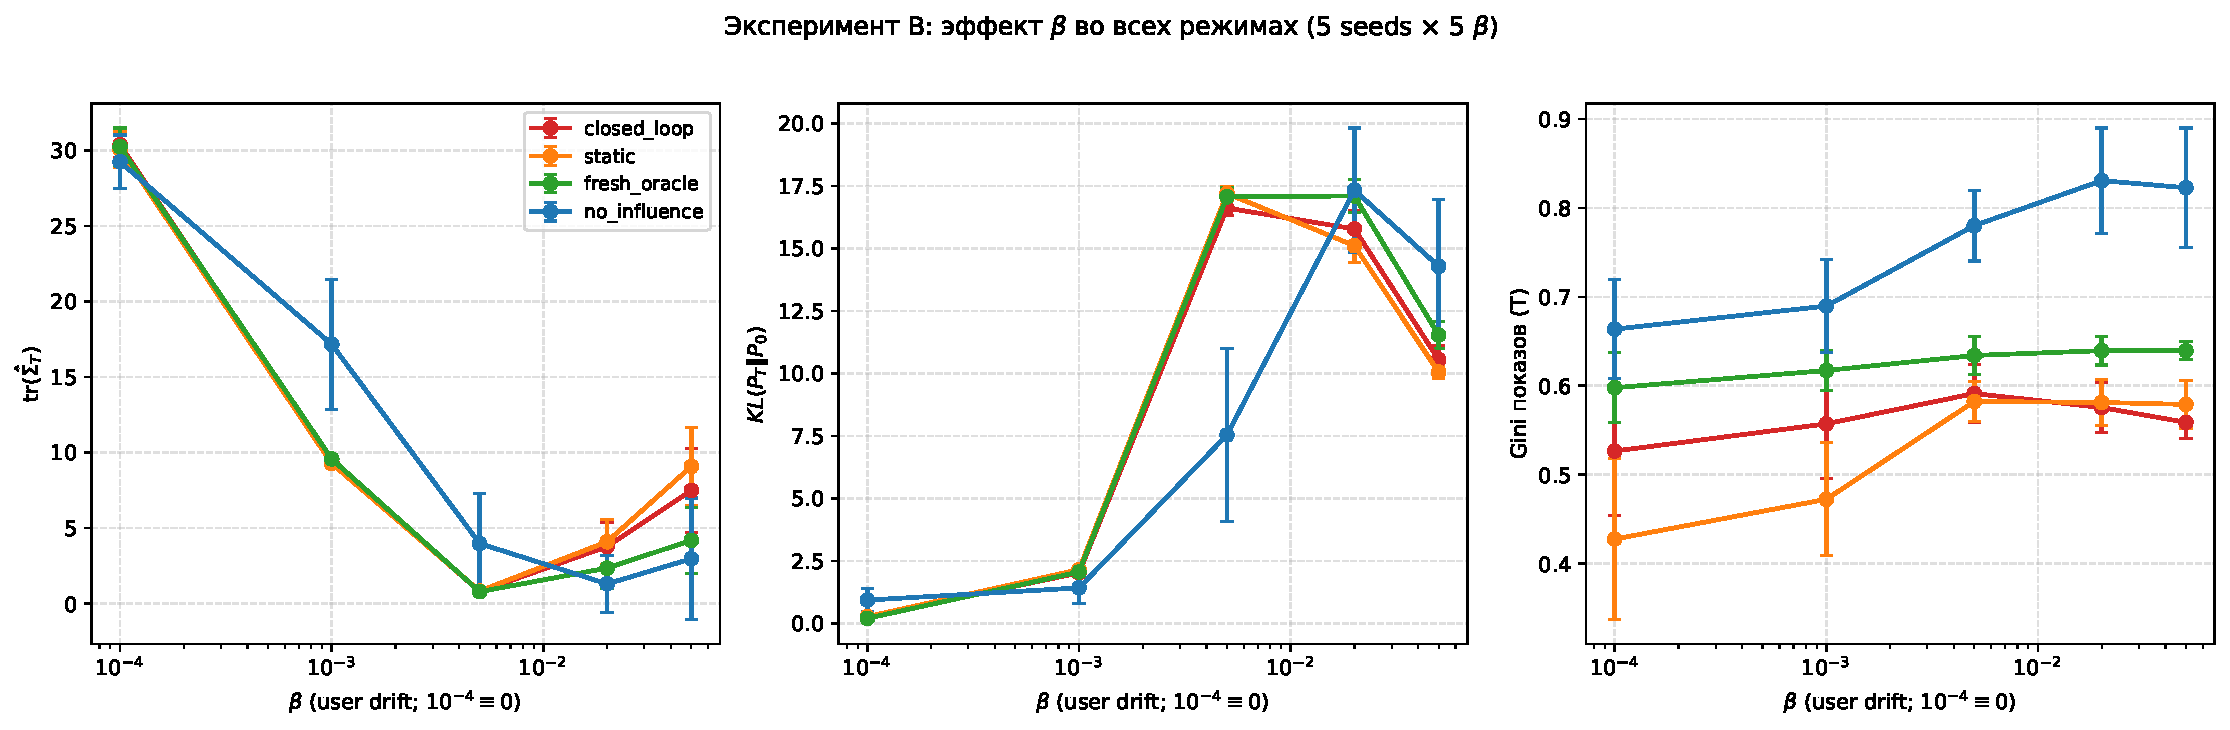
\includegraphics[width=0.85\textwidth]{figures/diagnostic/DIAG_B_beta_sweep_v2}
    \caption{Остаточное разнообразие $\operatorname{tr}\hat\Sigma$ после $T$ шагов
    как функция силы дрейфа $\beta$ для четырёх режимов. При $\beta=0$ стягивания
    нет ни в одном режиме; при $\beta>0$ оно наступает одинаково во всех режимах с
    $\alpha>0$, что подтверждает следствия~\ref{cor:no_beta}
    и~\ref{cor:universal}.}
    \label{fig:beta_sweep}
\end{figure}

При $\beta=0$ след ковариации сохраняется на уровне $\operatorname{tr}
\hat\Sigma\approx30$ во всех режимах, включая режим петли (рис.~\ref{fig:beta_sweep}),
что прямо подтверждает следствие~\ref{cor:no_beta}. При $\beta=0{,}005$
стягивание достигает максимума ($\operatorname{tr}\hat\Sigma\approx0{,}8$) во
всех режимах с $\alpha>0$. Дополнительный эксперимент со статической моделью при
варьировании $\alpha$ показывает, что уже при $\alpha\ge0{,}4$ стягивание
достигает уровня петли, то есть переобучение не является его источником.

\begin{figure}[H]
    \centering
    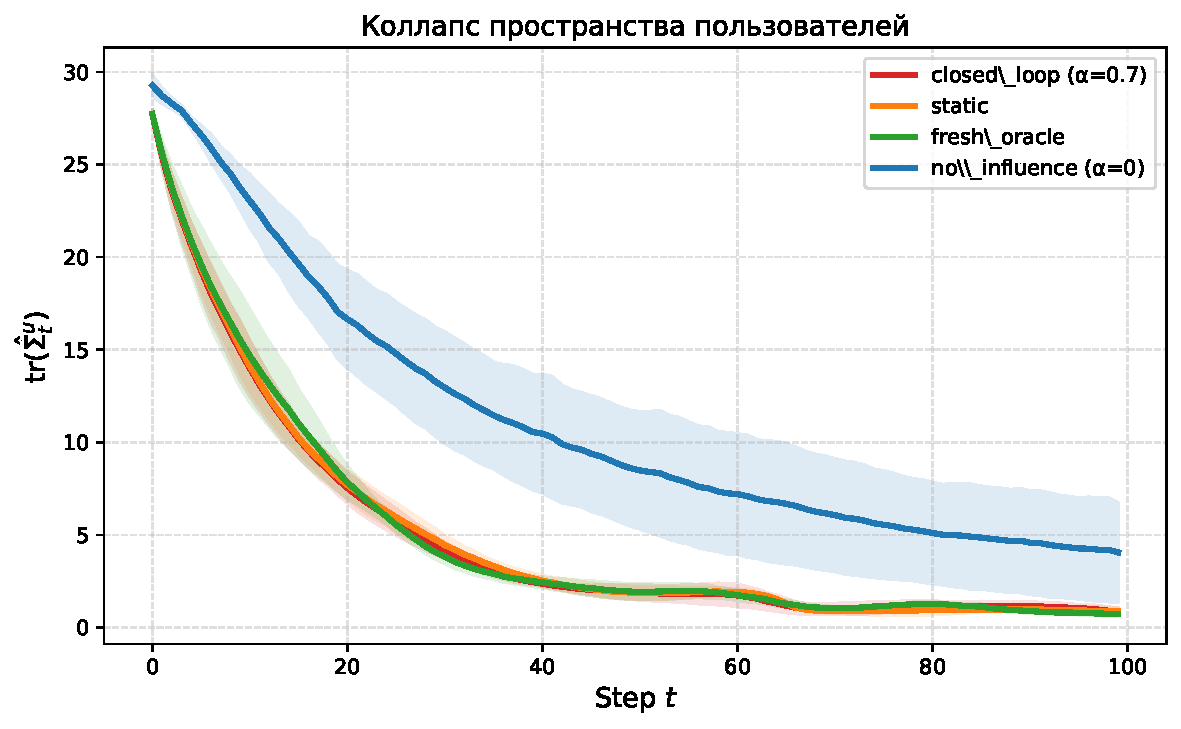
\includegraphics[width=\textwidth]{figures/H1_H3_trace_sigma}
    \caption{Динамика следа ковариации $\operatorname{tr}\hat\Sigma_t$ по четырём
    режимам. Стягивание наступает во всех режимах с дрейфом; режим без следования
    рекомендациям \texttt{no\_influence} стягивается слабее за счёт большего
    разброса показанного.}
    \label{fig:h1h3_trace}
\end{figure}

Численные итоги приведены в таблице~\ref{tab:h1h3}. Стягивание следа ковариации в
режиме петли составляет $-96{,}9\%$, в режиме \texttt{no\_influence}~---
$-86{,}1\%$; режимы \texttt{static} и \texttt{fresh\_oracle} дают близкий к петле
результат ($-96{,}8\%$ и $-97{,}4\%$), что согласуется со
следствием~\ref{cor:universal}: закон убывания общий для всех режимов с дрейфом.

\begin{table}[H]
    \caption{Итоговые метрики после $T=100$ шагов (среднее по $5$ запускам)}
    \label{tab:h1h3}
    \centering
    \begin{tabular}{lccc}
        \toprule
        Режим & $\mathrm{KL}(P_T\Vert P_0)$ & $\operatorname{tr}\hat\Sigma_T$ & $\Delta\operatorname{tr}$, \% \\
        \midrule
        \texttt{closed\_loop}  & $16{,}88$ & $0{,}865$ & $-96{,}9$ \\
        \texttt{static}        & $17{,}25$ & $0{,}878$ & $-96{,}8$ \\
        \texttt{fresh\_oracle} & $16{,}95$ & $0{,}723$ & $-97{,}4$ \\
        \texttt{no\_influence} & $\phantom{0}7{,}31$ & $4{,}06$ & $-86{,}1$ \\
        \bottomrule
    \end{tabular}
\end{table}

\subsection{$K$-модальная структура эхо-камер}
\label{subsec:exp_kmodal}

Теорема~\ref{thm:beta} применяется к каждому кластеру отдельно, поэтому при
$K>1$ ожидается формирование $K$ независимых зон стягивания при сохранении
межкластерного зазора. Гипотеза проверяется на сетке значений числа кластеров
$K\in\{1,2,4\}$ и межкластерного расстояния.

\begin{figure}[H]
    \centering
    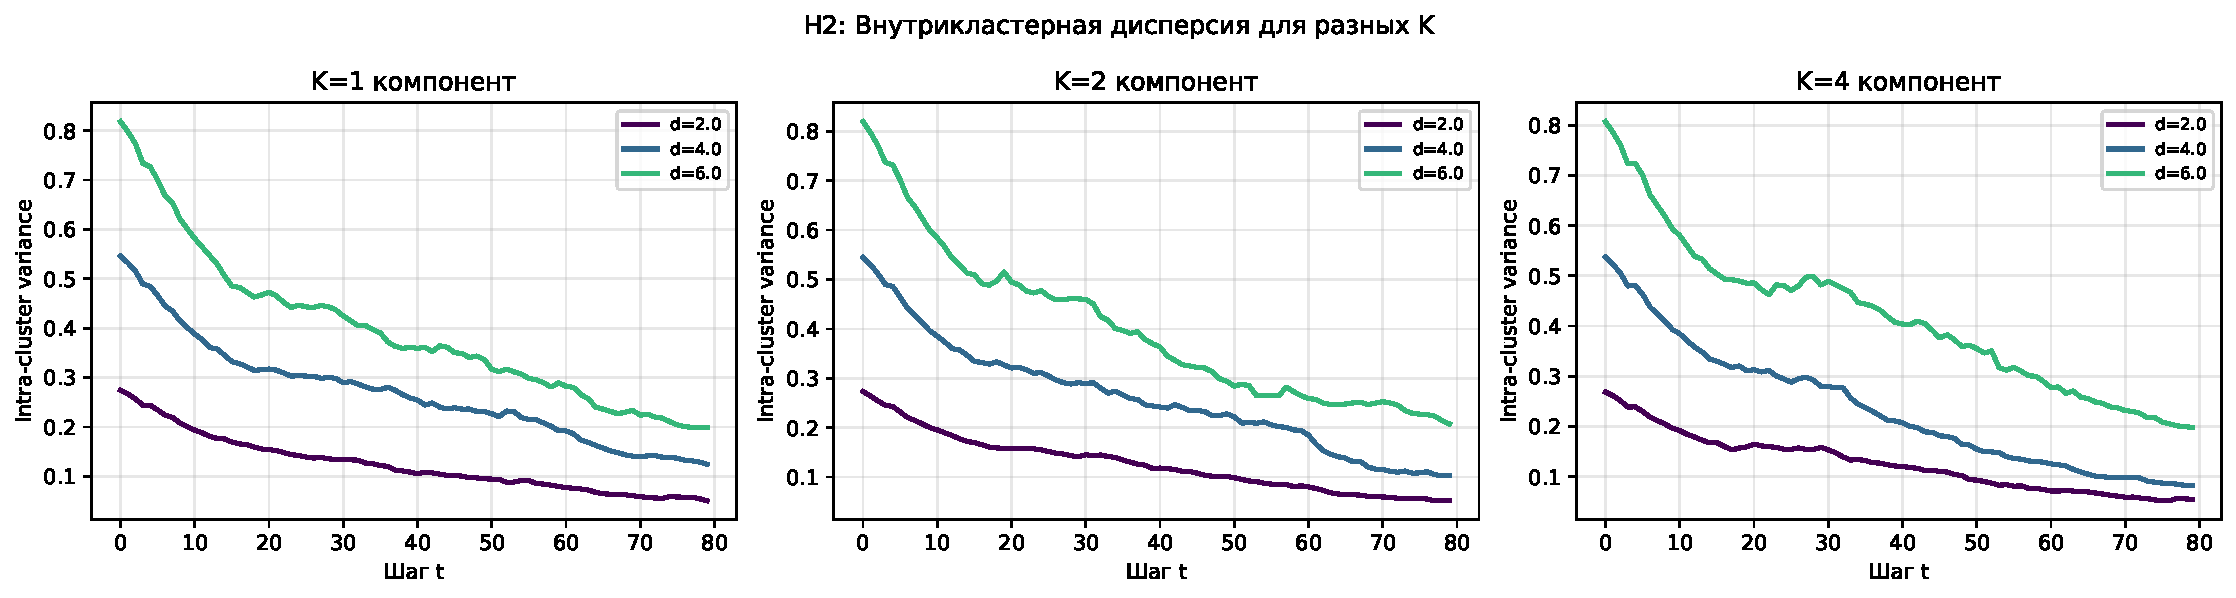
\includegraphics[width=\textwidth]{figures/H2_intra_cluster_variance}
    \caption{Внутрикластерная дисперсия во времени при $K\in\{1,2,4\}$ и трёх
    значениях межкластерного расстояния. Дисперсия убывает на $77$--$85\%$,
    быстрее при большем $K$.}
    \label{fig:h2_intra}
\end{figure}

Внутрикластерная дисперсия убывает на $77\%$ при $K=1$, на $81\%$ при $K=2$ и на
$85\%$ при $K=4$ (рис.~\ref{fig:h2_intra}); коэффициент силуэта при этом не
деградирует ($0{,}634\to0{,}677$ при $K=4$), то есть кластеры уплотняются, но не
сливаются. Скорость стягивания растёт с $K$: чем теснее объекты к пользователям
своего сегмента, тем эффективнее дрейф концентрирует эмбеддинги. Качественная
картина показана на PCA-снимках (рис.~\ref{fig:t3_pca}): облака сжимаются к
центроидам при сохранении расстояния между ними.

\begin{figure}[H]
    \centering
    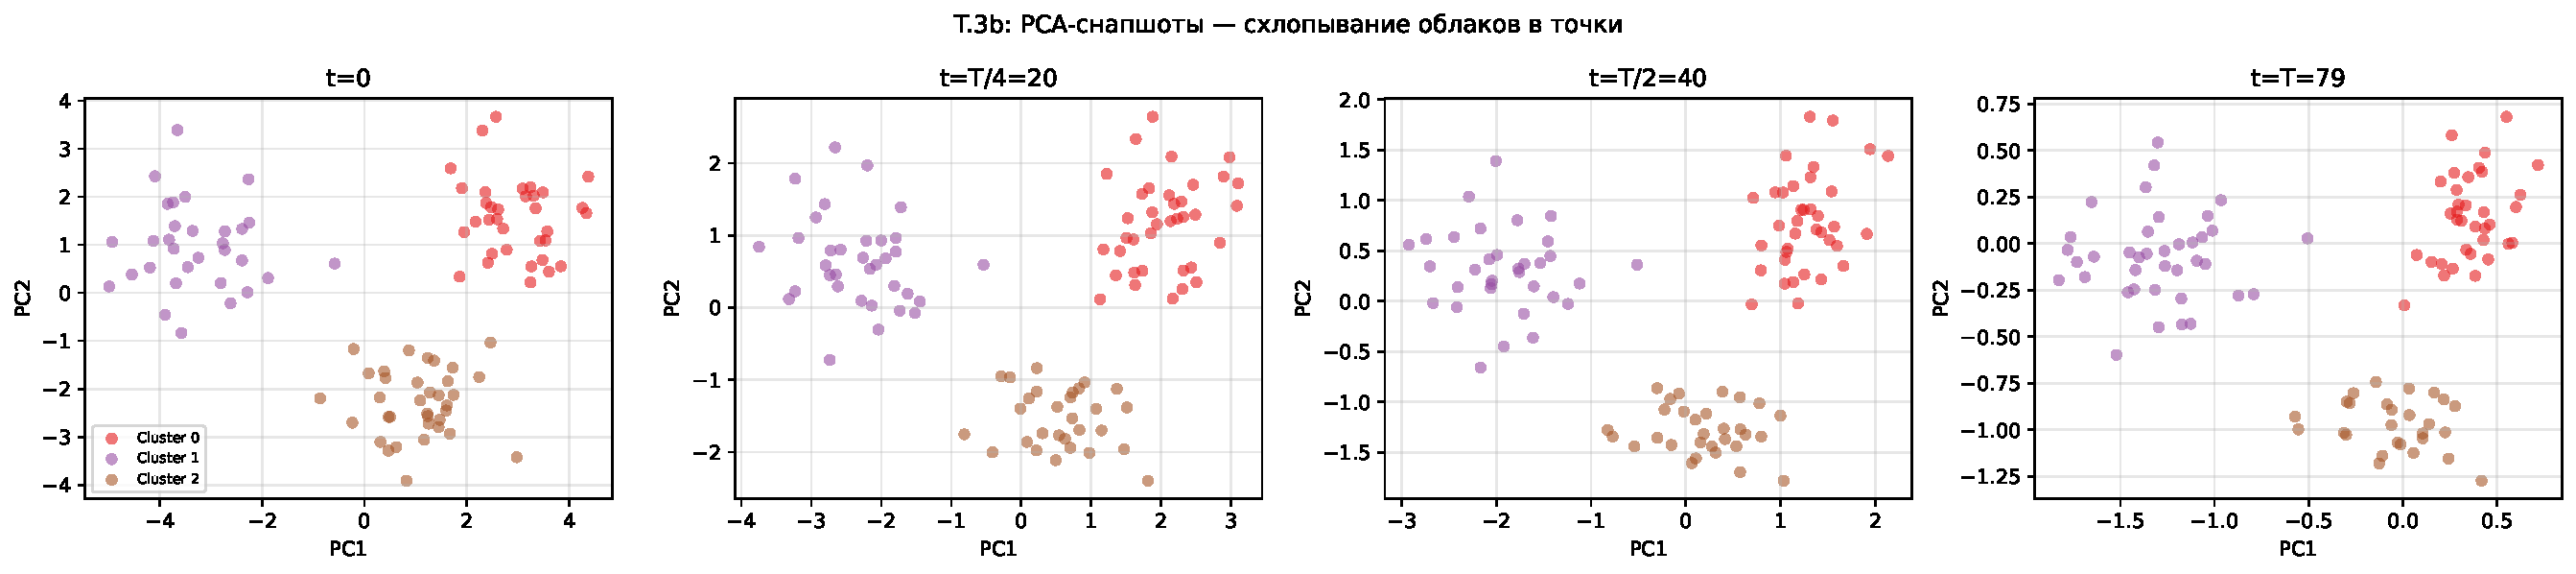
\includegraphics[width=\textwidth]{figures/T3_pca_snapshots}
    \caption{Снимки эмбеддингов (метод главных компонент) в моменты $t\in\{0,
    T/4, T/2, T-1\}$ при $K=3$; цвет~--- кластер. Стягивание персонализации внутри
    кластеров при сохранении межкластерного разделения.}
    \label{fig:t3_pca}
\end{figure}

\subsection{Геометрия стягивания}
\label{subsec:exp_geometry}

Ряд проверок уточняет геометрию предельного режима, предсказанного
Теоремой~\ref{thm:beta}. Спектральный радиус $\lambda_{\max}(\hat\Sigma_k)$
монотонно убывает для всех кластеров; для $23$ независимых начальных
распределений все траектории среднего следа монотонно убывают к нулю, что
подтверждает глобальность аттрактора. Внутрикластерный индекс Жаккара рекомендаций
растёт с $0{,}50$ до $0{,}86$ ($+71\%$): к концу горизонта пользователи одного
кластера получают почти одинаковые списки.

\begin{figure}[H]
    \centering
    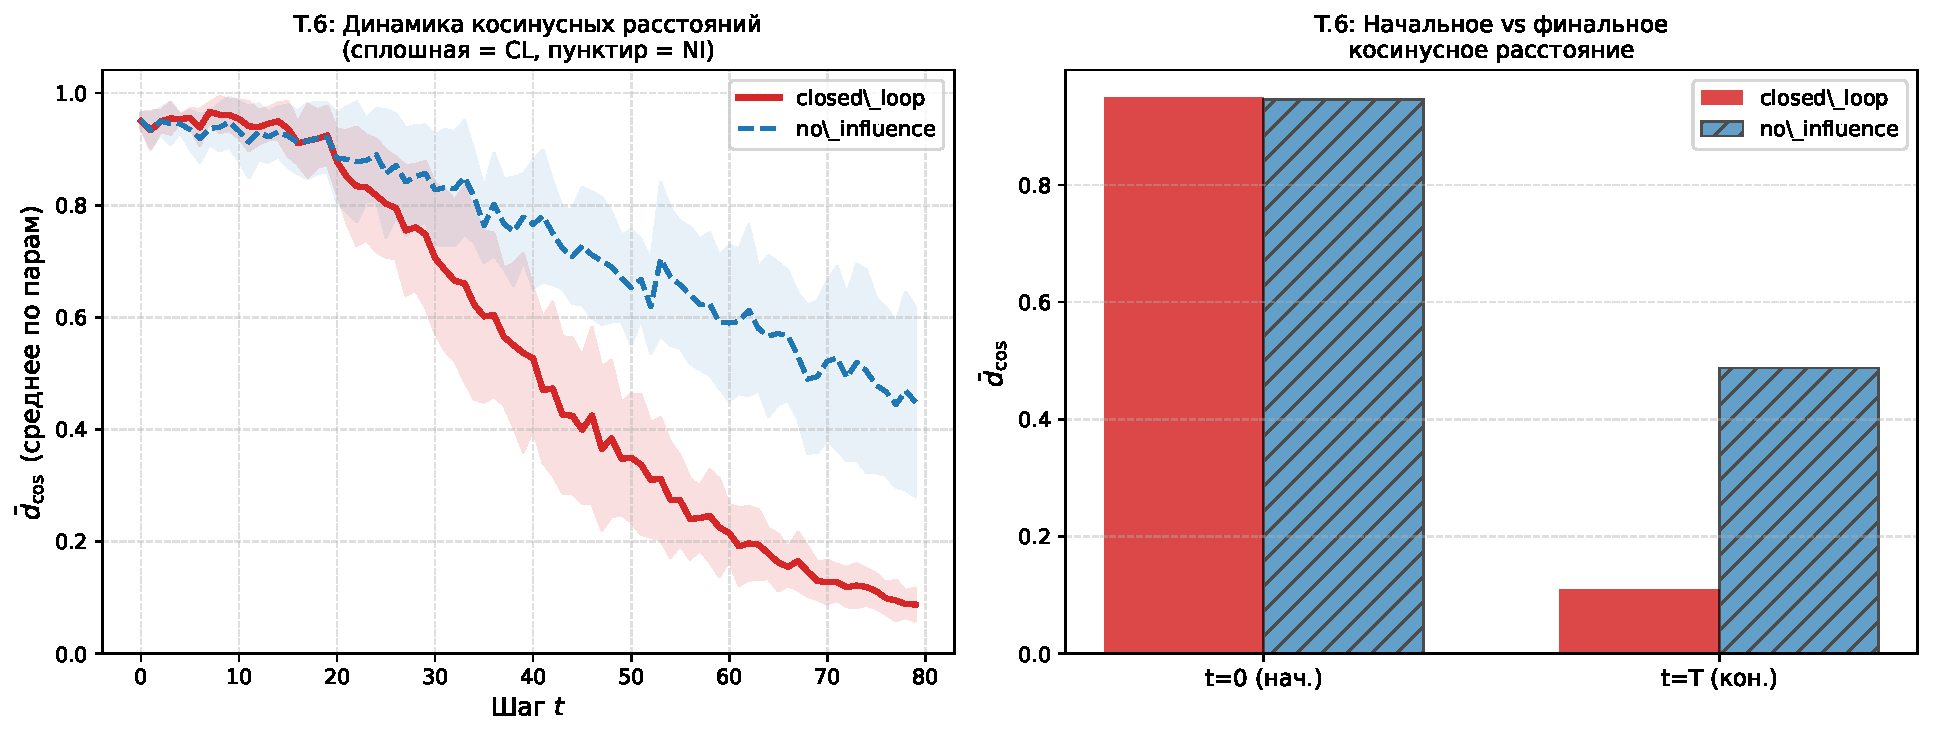
\includegraphics[width=0.9\textwidth]{figures/T6_cosine_distances}
    \caption{Среднее попарное косинусное расстояние между пользователями. В
    режиме петли эмбеддинги становятся почти коллинеарны ($d_{\cos}\approx0{,}11$),
    тогда как в \texttt{no\_influence} сохраняется существенное угловое
    разнообразие ($d_{\cos}\approx0{,}49$).}
    \label{fig:t6_cosine}
\end{figure}

Среднее попарное косинусное расстояние (рис.~\ref{fig:t6_cosine}) убывает в петле
в $4{,}4$ раза сильнее, чем в контрольном режиме, то есть кластер схлопывается к
почти одномерному подпространству вдоль направления доминирующего объекта.
Анализ фрагментации (рис.~\ref{fig:t7_frag}) показывает, что доля межкластерной
дисперсии $\eta^2$ в петле растёт ($0{,}33\to0{,}46$): аудитория всё чётче
распадается на изолированные сегменты.

\begin{figure}[H]
    \centering
    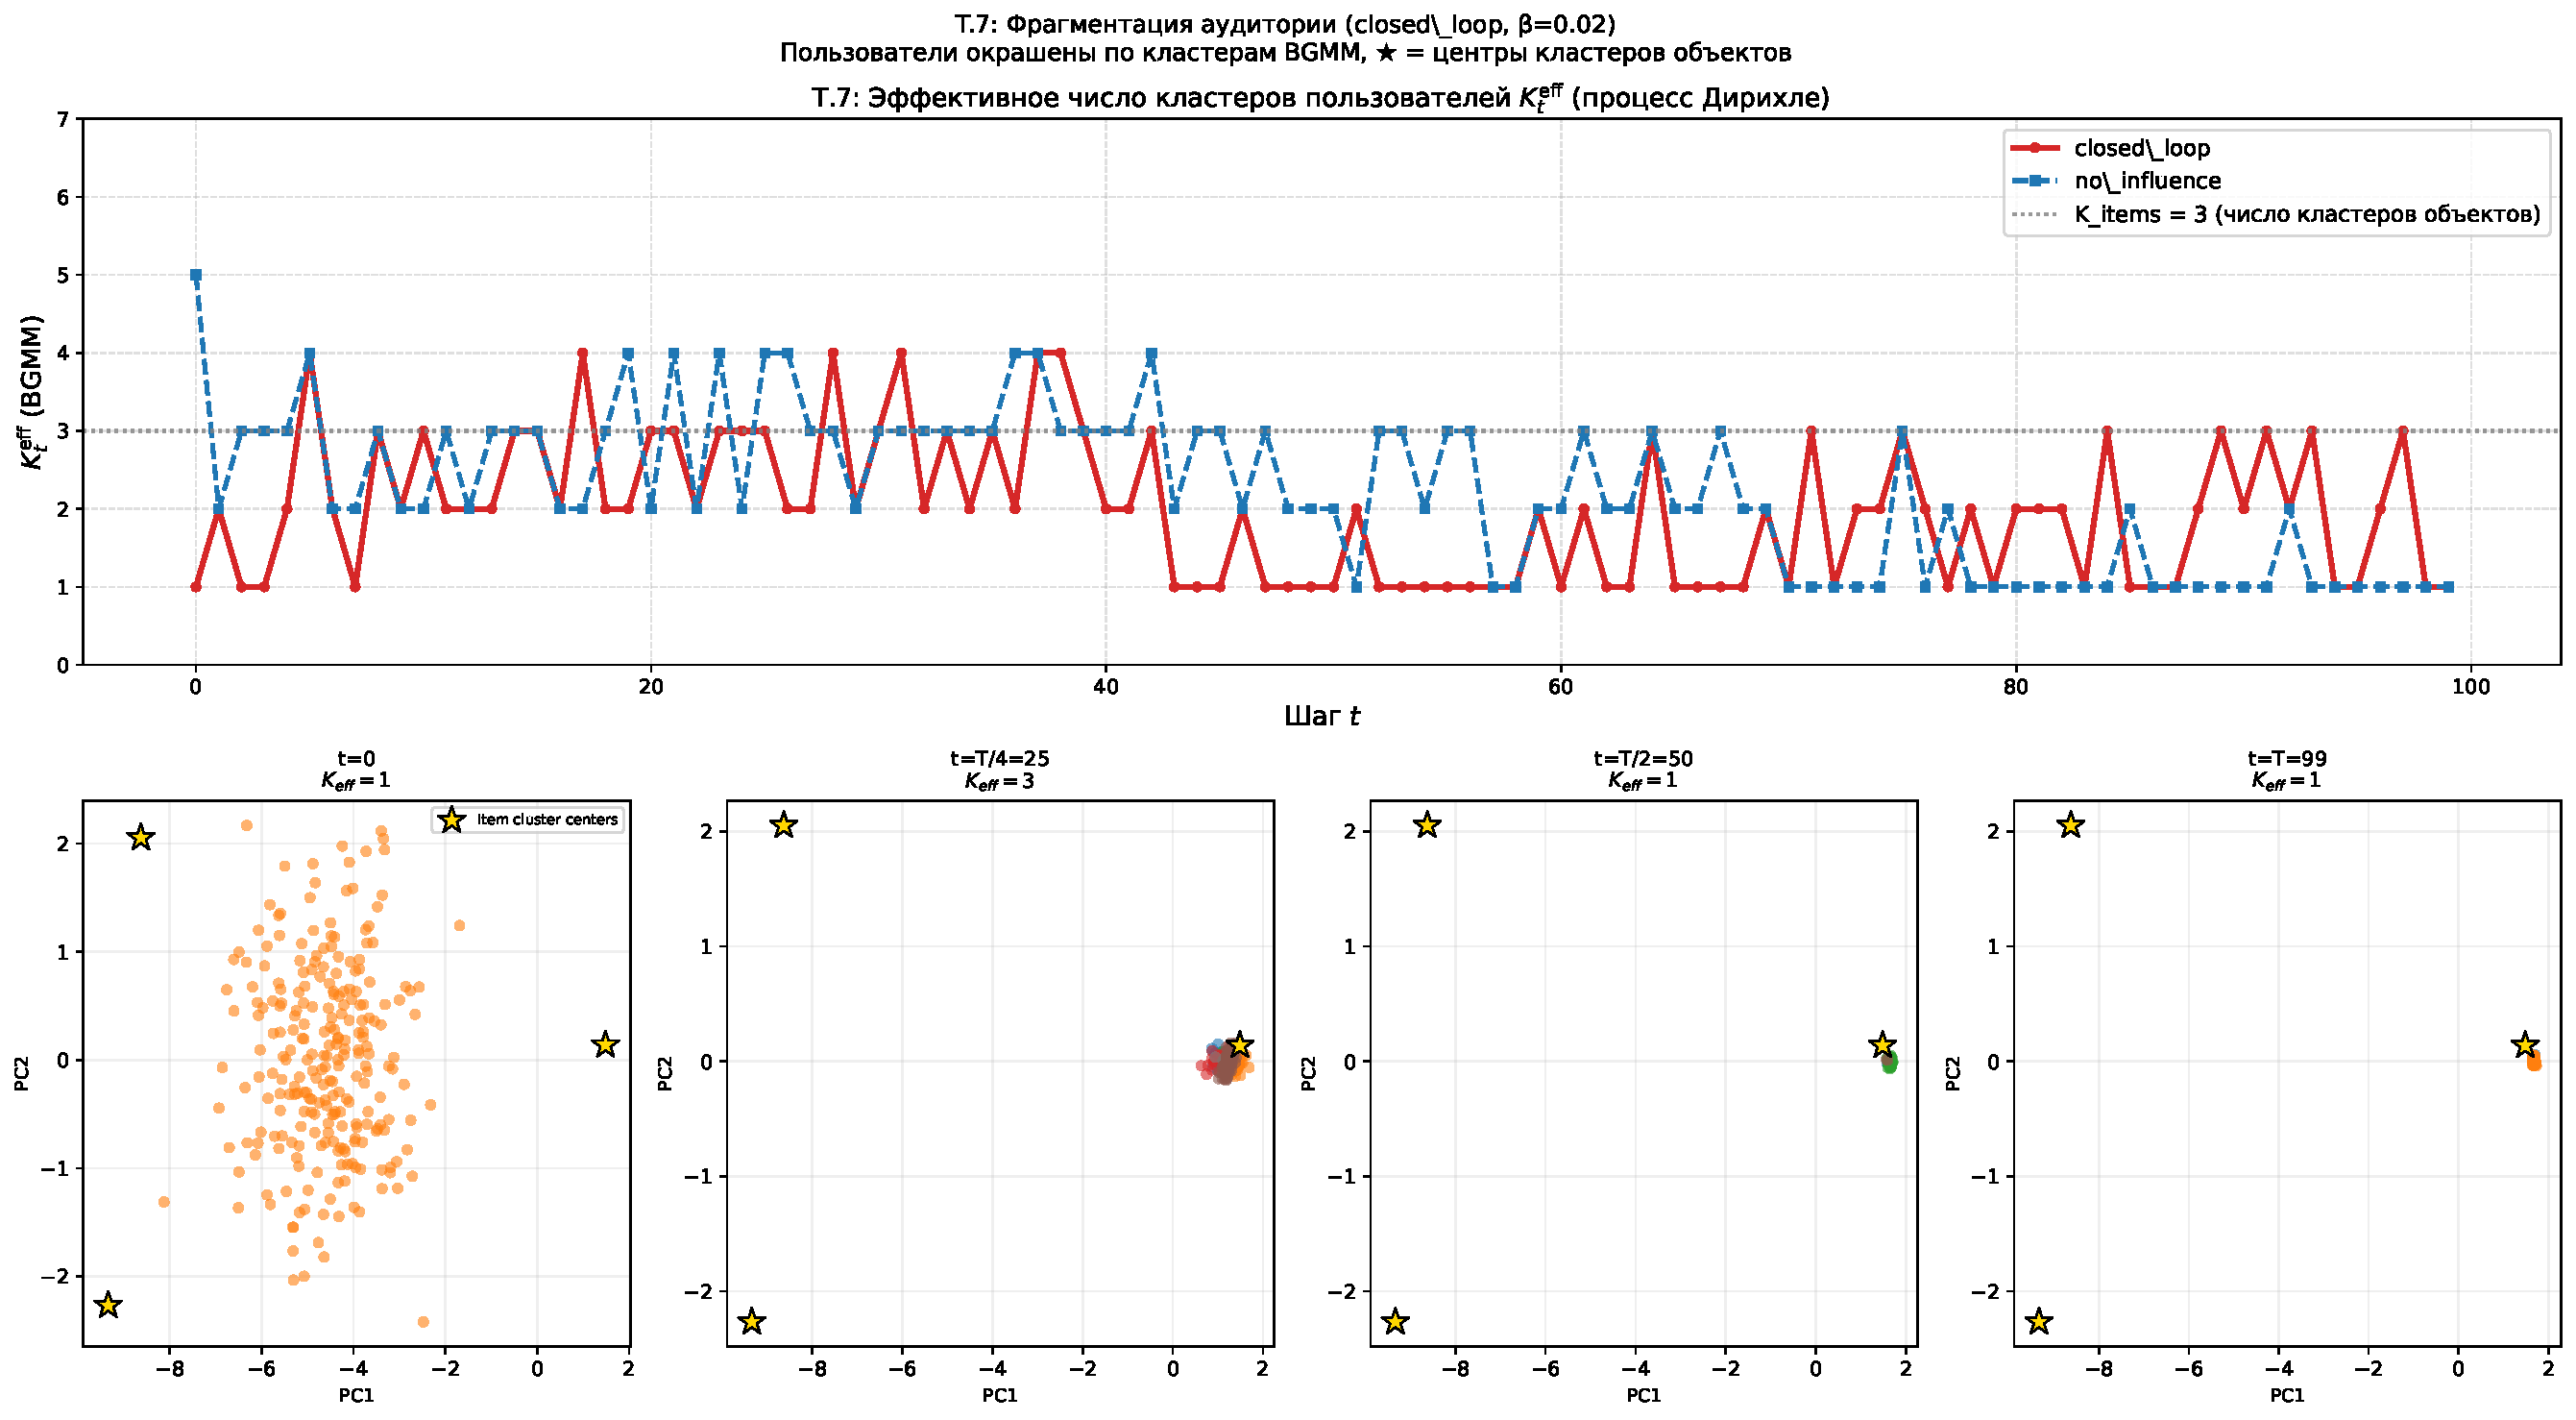
\includegraphics[width=0.8\textwidth]{figures/T7_fragmentation_dpmm}
    \caption{Доля межкластерной дисперсии $\eta^2$ во времени. В режиме петли рост
    выражен сильнее ($0{,}33\to0{,}46$), чем в \texttt{no\_influence}
    ($0{,}36\to0{,}40$): популяция фрагментируется на изолированные сообщества.}
    \label{fig:t7_frag}
\end{figure}

\subsection{Фазовая диаграмма стягивания}
\label{subsec:exp_phase}

Теорема~\ref{thm:beta} предсказывает, что граница стягивания определяется
произведением силы следования и активности. На сетке $8\times8$ по
$(\alpha,\rho)$ ($192$ запуска) измерялась остаточная доля дисперсии.

\begin{figure}[H]
    \centering
    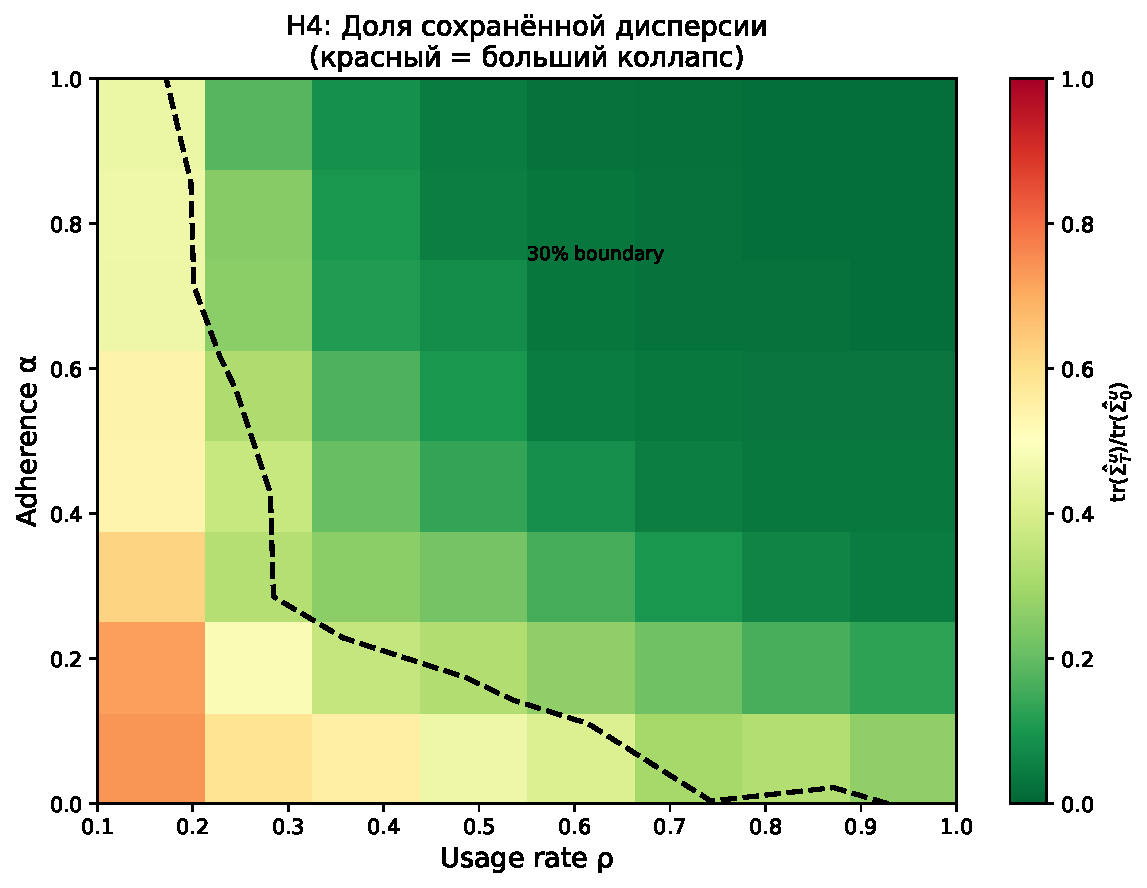
\includegraphics[width=\textwidth]{figures/H4_phase_diagram}
    \caption{Фазовая диаграмма остаточной доли дисперсии в координатах (сила
    следования $\alpha$, активность $\rho$). Граница стягивания определяется
    произведением $\alpha\cdot\rho$: чем оно больше, тем полнее стягивание.}
    \label{fig:h4_phase}
\end{figure}

При $\rho=1$ остаточная доля монотонно убывает с $0{,}268$ при $\alpha=0$ до
$0{,}018$ при $\alpha=1$ (рис.~\ref{fig:h4_phase}). Линии уровня диаграммы близки
к гиперболам $\alpha\rho=\mathrm{const}$, что согласуется с зависимостью
множителя $q=1-\beta\rho(2-\beta)$ и концентрации выдачи (через $\alpha$) от этих
двух параметров.

\subsection{Наблюдаемое и истинное качество}
\label{subsec:exp_quality}

Предложение~\ref{prop:self_reinforcement} предсказывает, что наблюдаемое качество
держится выше истинного на всём горизонте. Раздельное измерение качества (по
логам и по истинным вероятностям отклика) подтверждает это
(рис.~\ref{fig:h6_quality}):
наблюдаемое качество снижается с $0{,}754$ до $0{,}686$ ($-9\%$), истинное~--- с
$0{,}690$ до $0{,}662$ ($-4{,}1\%$), и наблюдаемое держится выше истинного во все
моменты. Самоподкрепляющееся слагаемое $\alpha\Delta_f$ завышает наблюдаемую
метрику ровно так, как предсказывает предложение~\ref{prop:self_reinforcement}.
По смыслу это тот же источник риска, который в литературе обсуждается как
смешение в логированных откликах и как причина для контрфактической или каузальной
интерпретации логов~\cite{bottou2013, sinha2016, krauth2022}.

\begin{figure}[H]
    \centering
    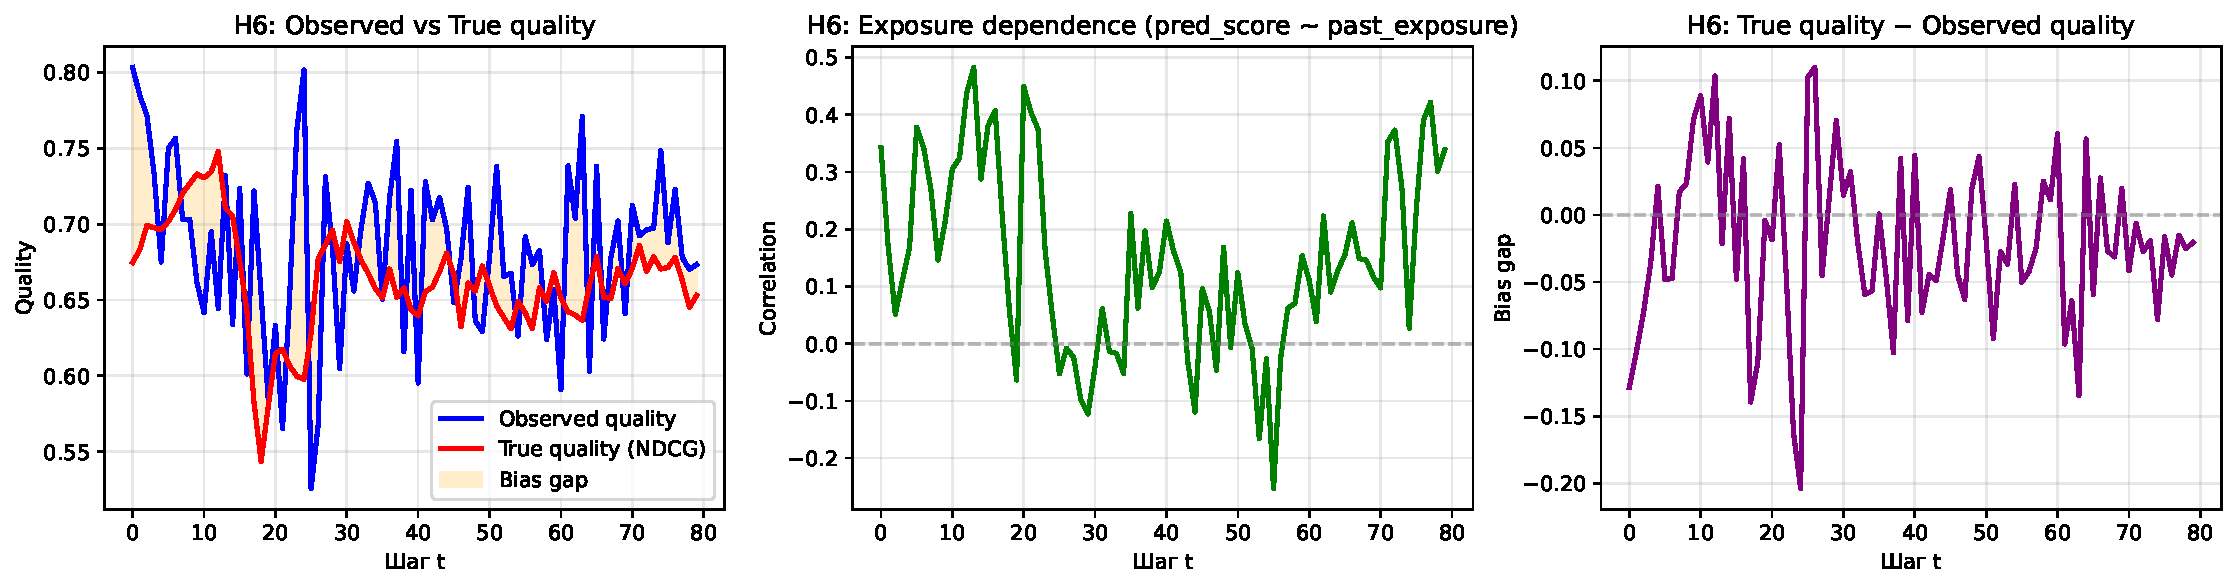
\includegraphics[width=\textwidth]{figures/H6_quality_gap}
    \caption{Наблюдаемое (по логам) и истинное (по вероятностям
    $\theta_t^{ij}$) качество во времени. Наблюдаемое держится выше истинного на
    всём горизонте, что подтверждает
    предложение~\ref{prop:self_reinforcement}.}
    \label{fig:h6_quality}
\end{figure}

\subsection{След петлевого канала в ковариации}
\label{subsec:exp_sensitivity}

Согласно Теореме~\ref{thm:loop}, переобучение оставляет отделимый след в форме
ковариации, а условием его появления служит различимость пользователей
$\lVert J_k\rVert\neq0$. Чтобы выделить этот след, измерялся разрыв между
режимами петли и заморозки при разных классах модели и способах инициализации
(факторный план $2\times3\times4\times30$ запусков). Такая диагностика близка к
идее отделять собственные предпочтения от влияния рекомендателя, но здесь
измеряется не восстановленный отклик, а геометрический след петли в ковариации
~\cite{sinha2016, pagan2023feedbackLoops}.

\begin{figure}[H]
    \centering
    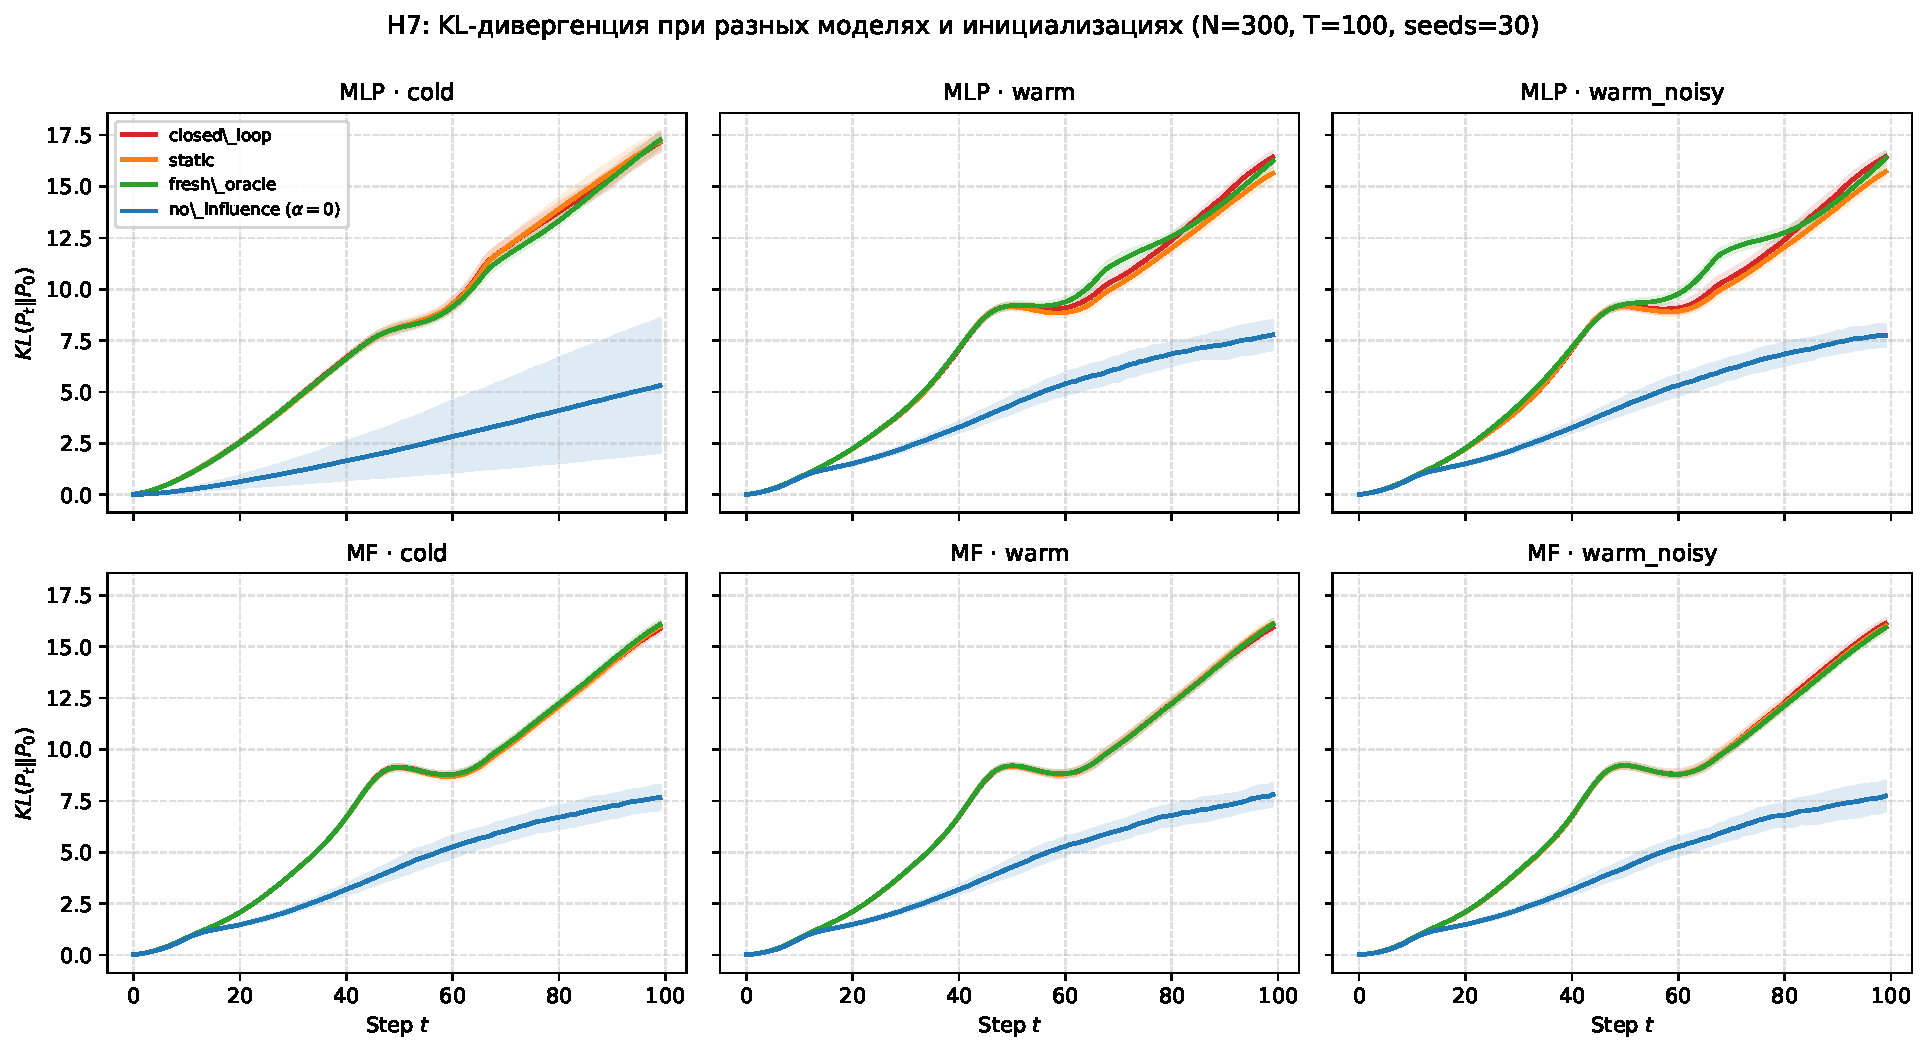
\includegraphics[width=\textwidth]{figures/H7_kl_grid}
    \caption{Разрыв $\mathrm{KL}$ между режимами петли и заморозки по классу
    модели и инициализации. Сигнал петли значим для предобученного MLP, где
    оценка существенно зависит от пользователя ($\lVert J_k\rVert\neq0$), и
    отсутствует при случайной инициализации.}
    \label{fig:h7_kl}
\end{figure}

При предобученной модели (тёплый старт), где $\lVert J_k\rVert\neq0$, разрыв
$\mathrm{KL}$ между петлёй и заморозкой значим и положителен, $+0{,}79$
($95\%$-й доверительный интервал $[0{,}64;0{,}95]$), а разрыв по следу ковариации
составляет $-0{,}16$ (рис.~\ref{fig:h7_kl}): петля даёт более глубокое и иначе
устроенное сжатие. При случайной инициализации, когда оценка почти не зависит от
пользователя, разрыв $\mathrm{KL}$ статистически незначим~--- в полном
согласии с условием активации $\lVert J_k\rVert\neq0$ из
раздела~\ref{subsec:metric}.

Решающую проверку предсказания Теоремы~\ref{thm:loop} о локализации следа даёт
разложение $\mathrm{KL}$ на слагаемое сдвига центра и дисперсионное слагаемое
(таблица~\ref{tab:dispersion}). Весь разрыв между петлёй и заморозкой
сосредоточен в дисперсионном слагаемом ($+0{,}788$), тогда как сдвиг центра
незначим ($+0{,}002$). Это прямо подтверждает, что петля действует на
\emph{ковариацию} предпочтений, а не на положение центров, как и предсказано
обсуждением Теоремы~\ref{thm:loop}.

\begin{table}[H]
    \caption{Разложение разрыва $\mathrm{KL}$ (петля минус заморозка) на слагаемые;
    среднее по $30$ запускам, в скобках $95\%$-й доверительный интервал}
    \label{tab:dispersion}
    \centering
    \begin{tabular}{lc}
        \toprule
        Слагаемое & Разрыв (петля $-$ заморозка) \\
        \midrule
        $\mathrm{KL}$ полное            & $+0{,}789\;[0{,}66;0{,}93]$ \\
        \quad сдвиг центра              & $+0{,}002\;[-0{,}01;0{,}01]$ \\
        \quad дисперсионное слагаемое   & $+0{,}788\;[0{,}66;0{,}93]$ \\
        $\operatorname{tr}\hat\Sigma$   & $-0{,}162\;[-0{,}22;-0{,}11]$ \\
        \bottomrule
    \end{tabular}
\end{table}

Границы активации петлевого канала уточняет эксперимент с варьированием числа
кластеров и баланса их весов (рис.~\ref{fig:h8_K}). При $K=1$ след петли
отсутствует, при $K\ge2$ значим (максимум $+0{,}79$ при $K=3$, далее убывает с
ростом $K$); при сильном перекосе весов сегментов сигнал также исчезает, так как
доминирующий кластер делает популяцию практически одномодальной. Это согласуется
с условием $K\ge2$ из итога главы~\ref{sec:Chapter3}.

\begin{figure}[H]
    \centering
    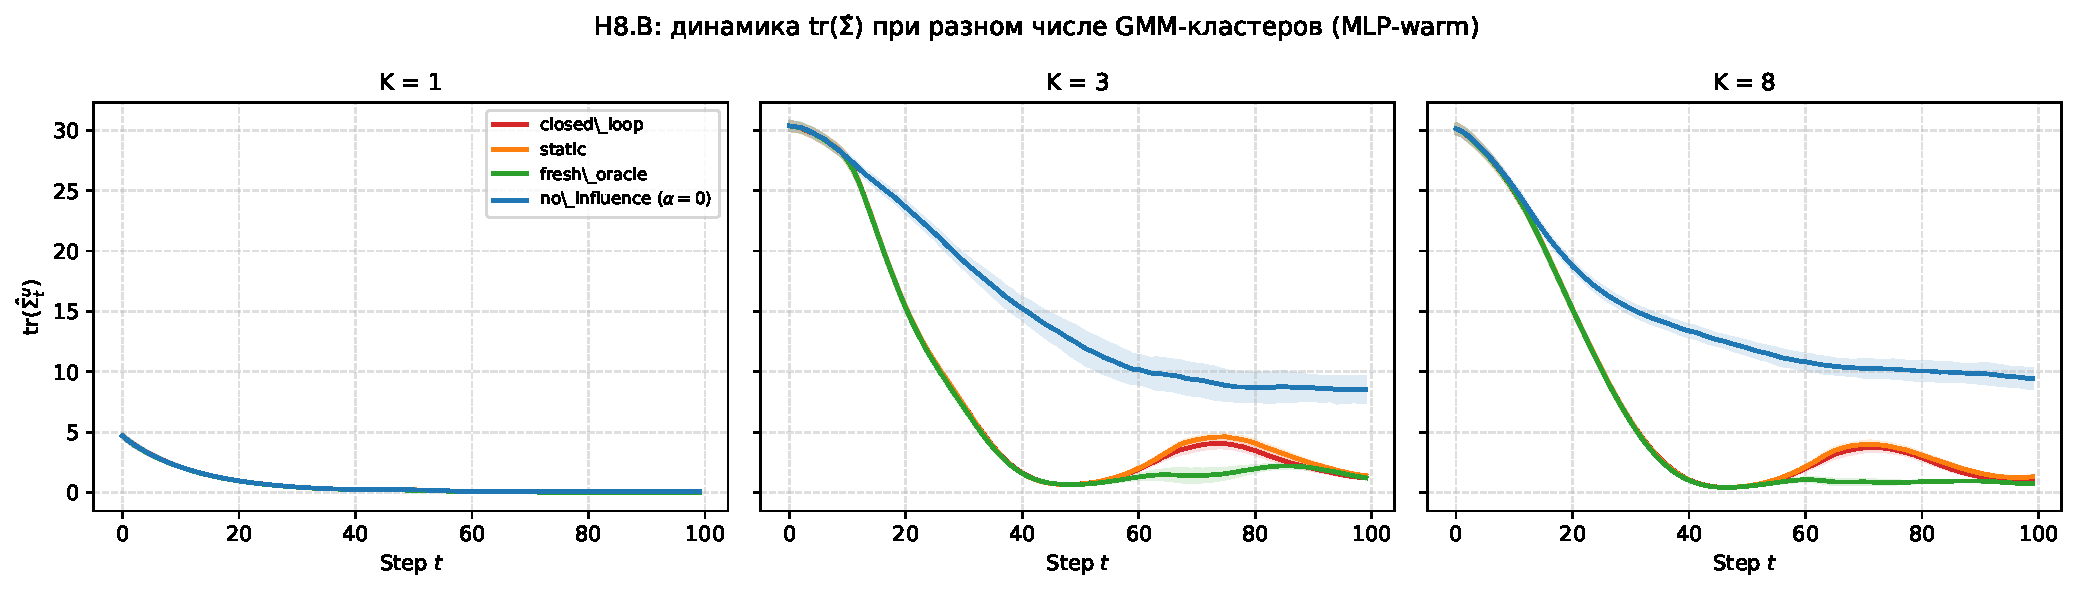
\includegraphics[width=\textwidth]{figures/H8_K_trajectories}
    \caption{Разрыв $\mathrm{KL}$ петля--заморозка в зависимости от числа
    сегментов $K$. Сигнал отсутствует при $K=1$ и значим при $K\ge2$, что
    подтверждает необходимость сегментной структуры для петлевого канала.}
    \label{fig:h8_K}
\end{figure}

% exp: code/experiments/diagnostic/exp_2026-06-15_kl_regularized_retrain.py
\subsection{Прямая проверка оператора переобучения}
\label{subsec:exp_klretrain}

Разложение расхождения локализует след петли в форме ковариации, но проверяет
Теорему~\ref{thm:loop} косвенно~--- через геометрию вкусов, а не через сам
оператор переобучения. Сама теорема опирается на
предположение~\eqref{eq:policy_improve}: переобучение действует как улучшение
политики с регуляризацией Кульбака--Лейблера, заостряя резкость $A_{k,t}$
(предложение~\ref{prop:sharpen}) и тем сужая ковариацию выдачи $C_{k,t}$.
Проверим это предсказание напрямую, заменив в контуре переобучение на сам
оператор~\eqref{eq:policy_improve} и измерив след ковариации показанного. Такая
проверка связывает модель с онлайн-оптимизацией по обратной связи и оптимальным
управлением замкнутой рекомендательной системой~\cite{mariano2026optimalControl,
chandrasekaran2026networkAware}.

В режиме петли кластерная политика инициализируется предобученной моделью
(резкость $A_{k,0}$) и на каждом шаге переобучения перевзвешивается по
Гиббсу, $S_k\leftarrow S_k+\kappa\,\widehat c_{k}$, где $\widehat c_k$~---
средний по кластеру логируемый отклик (смесь истинного отклика и
предсказания модели); в режиме заморозки политика неизменна. Прочие компоненты
контура сохранены, старты режимов совпадают (парный план, $10$ запусков,
$T=100$). Шаг переобучения $\kappa$ варьировался для проверки дозовой
зависимости.

Результаты (таблица~\ref{tab:klretrain}) подтверждают предсказание. Кривизна
отклика неотрицательна~--- предпосылка $H_{k,t}\succeq0$ выполнена во всех
кластерах,~--- а след ковариации выдачи в петле значимо меньше, чем при
заморозке, причём разрыв растёт по модулю с шагом переобучения $\kappa$
(от $-0{,}022$ при $\kappa=5$ до $-0{,}083$ при $\kappa=20$). Это прямо
воспроизводит следствие $\operatorname{tr}C_{k,t}^{\mathrm{closed}}\le
\operatorname{tr}C_{k,t}^{\mathrm{stat}}$ из обсуждения
Теоремы~\ref{thm:loop}: под её собственным оператором переобучение заостряет
выдачу, и тем сильнее, чем интенсивнее переобучение.

\begin{table}[H]
    \caption{Прямая проверка оператора переобучения~\eqref{eq:policy_improve}:
    разрыв следа ковариации выдачи $\operatorname{tr}C$ между режимами петли и
    заморозки; среднее по $10$ запускам, в скобках $95\%$-й доверительный интервал}
    \label{tab:klretrain}
    \centering
    \begin{tabular}{lc}
        \toprule
        Величина & Значение \\
        \midrule
        Кривизна отклика $H_{k,t}\succeq0$ (доля кластеров) & $100\%$ \\
        $\operatorname{tr}C$, петля $-$ заморозка ($\kappa=5$)  & $-0{,}022\;[-0{,}027;-0{,}017]$ \\
        $\operatorname{tr}C$, петля $-$ заморозка ($\kappa=20$) & $-0{,}083\;[-0{,}103;-0{,}064]$ \\
        \bottomrule
    \end{tabular}
\end{table}

Проверка относится к идеализированному оператору~\eqref{eq:policy_improve}. В
промышленных системах переобучение минимизирует существенно более сложную
функцию потерь~--- бинарную кросс-энтропию глубокой модели и её варианты,~---
оператор которой не сводится к чистому улучшению политики, и заострение выдачи в
таком режиме достигается труднее. Поэтому приведённый результат подтверждает
механизм Теоремы~\ref{thm:loop} в рамках её модельного допущения о форме
переобучения, оставляя количественную силу эффекта в реальных архитектурах
предметом дальнейшего изучения.

% exp: code/experiments/diagnostic/exp_2026-06-15b_kl_risk_gap.py
\subsection{Рост расхождения и надёжность офлайн-метрик}
\label{subsec:exp_klgap}

Предложение~\ref{prop:pinsker} ограничивает разрыв между наблюдаемым и истинным
качеством расхождением $\overline{\mathrm{KL}}_t$ между загрязнённым и истинным
откликом. Проверим, как $\overline{\mathrm{KL}}_t$ ведёт себя в контуре и
выполняется ли граница. На каждом шаге по показанным парам (распределение показов $\mu_t$)
измерялись $\overline{\mathrm{KL}}_t$, завышение метрики
$Q^{\mathrm{obs}}-Q^{\mathrm{true}}$ (наблюдаемый и истинный CTR показанного) и
граница Пинскера; режимы петли, заморозки и без влияния, $8$ запусков, $T=100$.
Такой эксперимент важен именно для офлайн-оценивания: стандартные метрики
ранжирования зависят от того, какие пары пользователь--объект были показаны, и
поэтому могут терять связь с истинной полезностью при смещённом распределении показов
~\cite{krichene2020, stoecker2025biasMitigation}.

\begin{figure}[H]
    \centering
    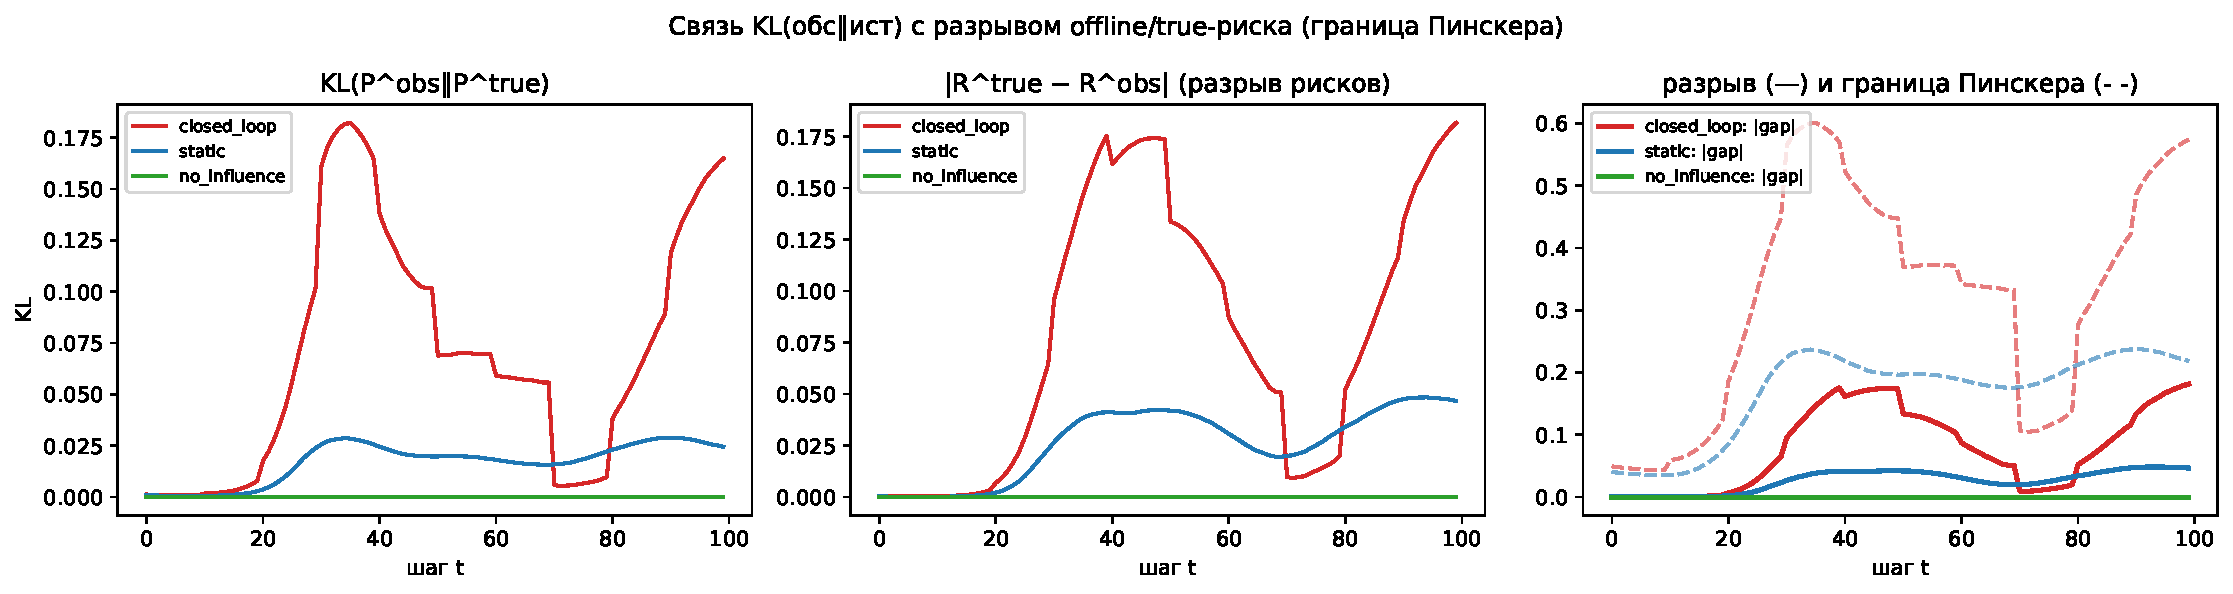
\includegraphics[width=\textwidth]{figures/diagnostic/DIAG_kl_risk_gap}
    \caption{Расхождение $\overline{\mathrm{KL}}_t$ между наблюдаемым и истинным
    откликом (слева), разрыв качества $|Q^{\mathrm{obs}}-Q^{\mathrm{true}}|$ (в
    центре) и его сравнение с границей Пинскера (справа, штрих) по трём режимам. В
    режиме петли расхождение и разрыв растут со шагом контура; в режиме без влияния
    ($\alpha=0$) загрязнения нет.}
    \label{fig:kl_risk_gap}
\end{figure}

Результаты (рис.~\ref{fig:kl_risk_gap}, таблица~\ref{tab:klgap}) подтверждают
предсказание. В режиме петли $\overline{\mathrm{KL}}_t$ растёт со шагом контура
(с почти нуля до $0{,}17$), завышение метрики увеличивается синхронно~--- до
$+0{,}18$ (наблюдаемый CTR $0{,}92$ против истинной релевантности $0{,}74$),~--- и
величина разрыва тесно следует за $\sqrt{\overline{\mathrm{KL}}_t}$ (коэффициент
корреляции $0{,}93$). Граница Пинскера выполняется на каждом шаге. Эффект
специфичен для переобучения: при заморозке рост $\overline{\mathrm{KL}}$ примерно
впятеро слабее (разрыв петля$-$заморозка по $\overline{\mathrm{KL}}$ значим,
$+0{,}14$, доверительный интервал $[0{,}13;0{,}15]$), а в режиме без влияния
загрязнения нет и $\overline{\mathrm{KL}}\equiv0$.

\begin{table}[H]
    \caption{Расхождение наблюдаемого и истинного отклика и разрыв качества на
    горизонте $t=T$; среднее по $8$ запускам}
    \label{tab:klgap}
    \centering
    \begin{tabular}{lcc}
        \toprule
        Режим & $\overline{\mathrm{KL}}_T$ & $|Q^{\mathrm{obs}}-Q^{\mathrm{true}}|_T$ \\
        \midrule
        \texttt{closed\_loop}  & $0{,}165$ & $0{,}182$ \\
        \texttt{static}        & $0{,}024$ & $0{,}047$ \\
        \texttt{no\_influence} & $0{,}000$ & $0{,}000$ \\
        \bottomrule
    \end{tabular}
\end{table}

По мере работы контура наблюдаемое качество расходится с истинным не быстрее, чем
позволяет $\overline{\mathrm{KL}}_t$, и поскольку переобучение на собственных
логах увеличивает это расхождение, офлайн-метрики перестают быть надёжным
индикатором реальной пользы~--- в количественном согласии с
Предложением~\ref{prop:pinsker}.

\subsection{Эксперименты на реальных данных}
\label{subsec:exp_real}

Для проверки переносимости выводов использован набор данных
\texttt{MovieLens-20M}~\cite{movielens20m}. В первой постановке синтетический
генератор пользователей заменён эмпирическим, восстановленным по матрице оценок
($500\times500$ после фильтрации, $d=16$, матричная факторизация, $3$ запуска);
прочие компоненты контура сохранены. Результаты воспроизводят синтетические:
$\operatorname{tr}\hat\Sigma$ в петле равен $0{,}174$ против $0{,}339$ в
\texttt{no\_influence}, а $\mathrm{KL}$ составляет $34{,}5$ против $19{,}7$
(разрыв $1{,}75$ раза), причём с более выраженным разделением режимов
(рис.~\ref{fig:real_ml}).
Использование MovieLens здесь не предполагает, что реальные логи являются
нейтральной выборкой предпочтений: напротив, именно такие исторические данные
мотивируют методы деконволюции и каузальной коррекции петли обратной связи
~\cite{sinha2016, chaney2018, krauth2022}.

\begin{figure}[H]
    \centering
    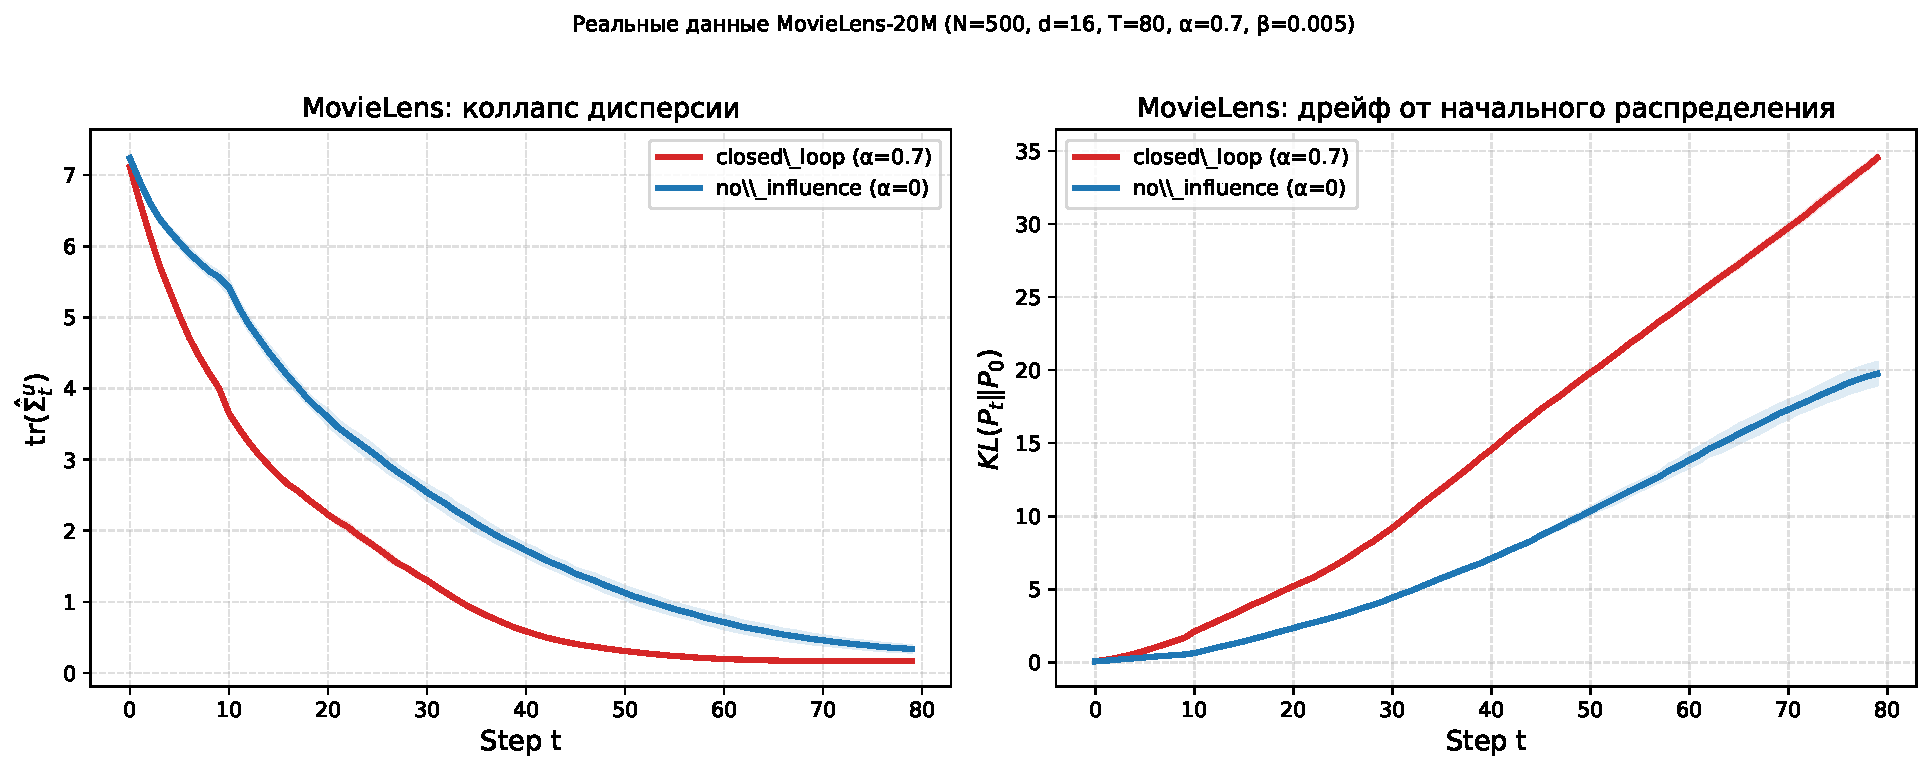
\includegraphics[width=\textwidth]{figures/real_data_movielens}
    \caption{Динамика $\mathrm{KL}(P_t\Vert P_0)$ и $\operatorname{tr}\hat\Sigma_t$
    на \texttt{MovieLens-20M} с эмпирическим генератором пользователей. Эффект
    воспроизводится вне синтетической среды.}
    \label{fig:real_ml}
\end{figure}

Во второй постановке коллапс наблюдается непосредственно в распределении
рекомендаций, без обращения к дрейфу эмбеддингов: модель в режиме петли
дообучается на собственных списках top-$L$ ($3000\times3000$, $d=32$, $L=10$,
$17$ квартальных окон). Покрытие каталога падает с $0{,}68$ до $0{,}24$, а
коэффициент Джини частот рекомендаций растёт с $0{,}67$ до $0{,}91$
(рис.~\ref{fig:collapse_direct}); в контрольном режиме без переобучения изменения
отсутствуют. Спустя моделируемый год система рекомендует втрое меньшую долю
каталога, что подтверждает выводы на уровне работы системы.

\begin{figure}[H]
    \centering
    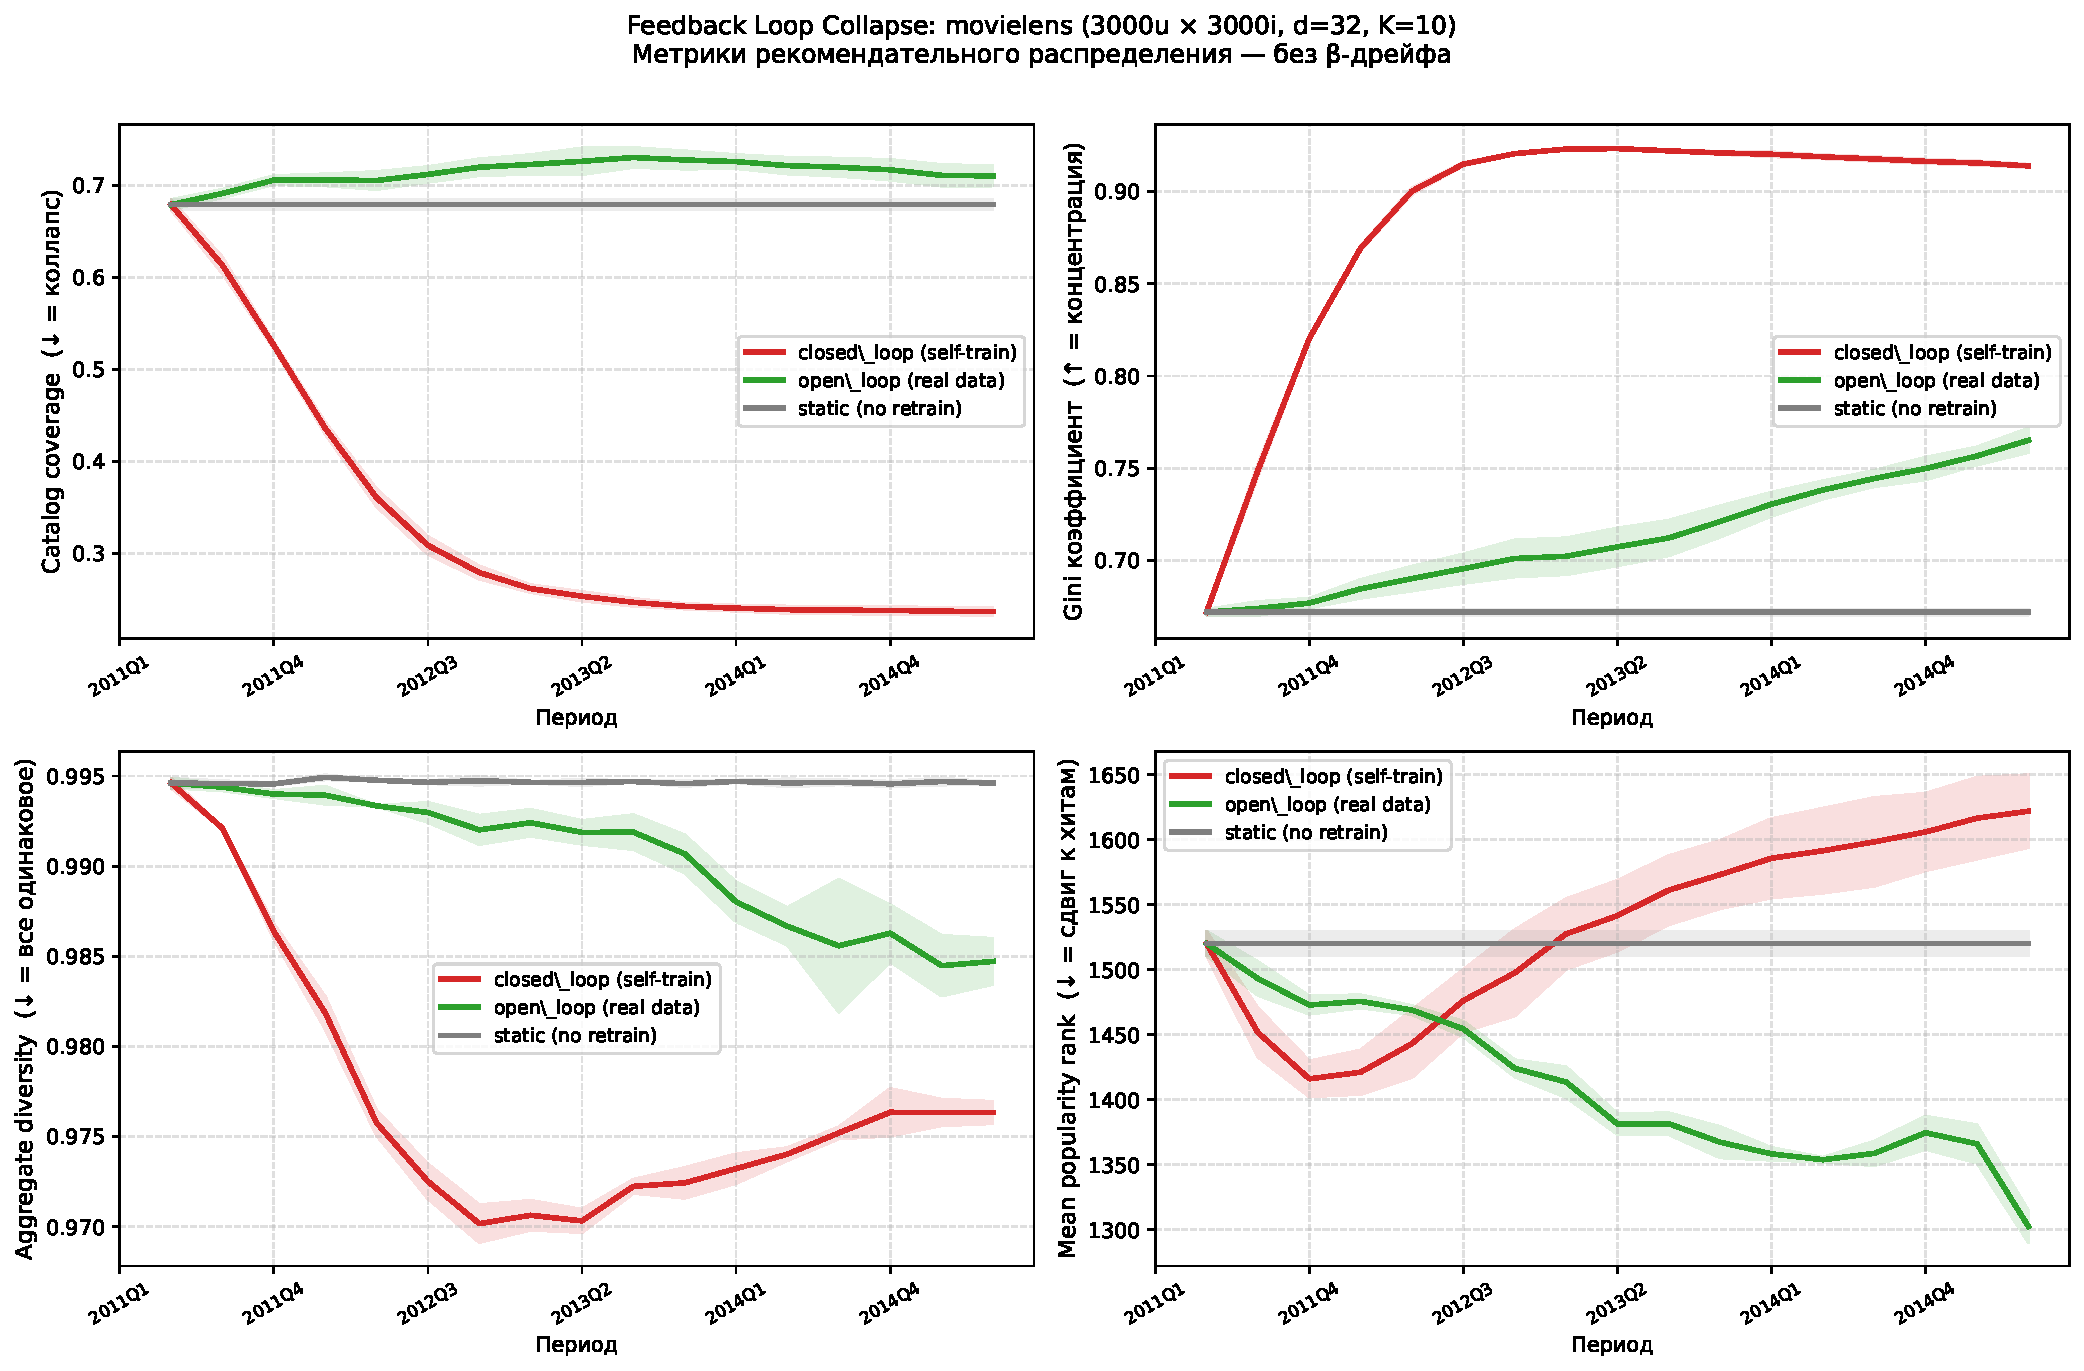
\includegraphics[width=\textwidth]{figures/collapse_direct_movielens}
    \caption{Прямое измерение стягивания распределения рекомендаций на
    \texttt{MovieLens-20M}: покрытие каталога, коэффициент Джини и разнообразие по
    трём режимам. В режиме петли покрытие падает более чем вдвое; контрольные
    режимы стабильны.}
    \label{fig:collapse_direct}
\end{figure}

Третья постановка проверяет само допущение о дрейфе предпочтений~\eqref{eq:drift}:
до сих пор сила дрейфа $\beta$ задавалась как параметр модели и из данных не
измерялась. В пространстве жанровых тегов \texttt{genome} ($1128$ признаков,
выведенных из содержания фильмов и независимых от поведенческих эмбеддингов;
сжато методом главных компонент до $20$ измерений) для каждого пользователя
строилась временная траектория центроидов потребления по последовательным окнам
просмотров. К ней применялась модель пространства состояний типа «случайное
блуждание с шумом», в которой стационарность потребления отвечает $\beta=0$, а
отношение дисперсии дрейфа к дисперсии внутриоконного шума даёт оценку
$\hat\beta=\sigma_\nu/\sigma_\varepsilon$. На $9{,}9$~млн положительных оценок
(порог $\ge 4$, $47{,}9$~тыс. пользователей) оценка дрейфа в $15$--$21$ раз
превосходит контрольное значение, полученное при перестановке порядка окон, по
всем $20$ компонентам, что свидетельствует о значимой нестационарности
предпочтений во времени. Полученная верхняя граница по наблюдательным данным на силу
дрейфа за один отклик составляет порядка $0{,}04$--$0{,}08$, внутри которой
используемое в симуляции значение $\beta=0{,}005$ оказывается консервативным.
Поскольку без экзогенной вариации показов рекомендательно-индуцированный
дрейф неотделим от автономной эволюции вкусов, эта оценка является верхней
границей; её каузальное уточнение намечено в главе~\ref{sec:Chapter6}.

\subsection{Сводка: теория и эксперимент}
\label{subsec:exp_summary}

Таблица~\ref{tab:theory_exp} сопоставляет теоретические утверждения с их
численным подтверждением. Все ключевые предсказания обеих теорем подтверждены,
в том числе на реальных данных.

\begin{table}[H]
    \caption{Соответствие теоретических утверждений и эксперимента}
    \label{tab:theory_exp}
    \centering
    \begin{tabular}{p{6.2cm}p{3.2cm}p{4.2cm}}
        \toprule
        Утверждение & Эксперимент & Результат \\
        \midrule
        Предложение~\ref{prop:self_reinforcement}: наблюдаемое выше истинного &
        качество, рис.~\ref{fig:h6_quality} & $0{,}69\!\to\!0{,}66$ ниже
        $0{,}75\!\to\!0{,}69$ \\
        Теорема~\ref{thm:beta}: нет стягивания при $\beta=0$ &
        варьирование $\beta$ & $\operatorname{tr}\hat\Sigma\approx30$ \\
        Следствие~\ref{cor:universal}: универсальность по режиму &
        режимы \texttt{static}/\texttt{oracle} & спад $\approx97\%$ \\
        Теорема~\ref{thm:beta}: монотонность по $\alpha\rho$ &
        фазовая диаграмма & $0{,}27\to0{,}02$ \\
        Теорема~\ref{thm:beta}: глобальный аттрактор &
        $23$ инициализации & все $\to0$ \\
        Теорема~\ref{thm:loop}: след петли при $\lVert J_k\rVert\neq0$ &
        тёплый старт MLP & $\operatorname{tr}$ $-0{,}16$, $\mathrm{KL}$ $+0{,}79$ \\
        Теорема~\ref{thm:loop}: след в ковариации, не в центре &
        разложение $\mathrm{KL}$ & дисп. $+0{,}79$, центр $+0{,}00$ \\
        Условие $K\ge2$ & варьирование $K$ & $K{=}1$: нет; $K\ge2$: есть \\
        Перенос на реальные данные & \texttt{MovieLens-20M} &
        $\operatorname{tr}$ $0{,}17$ vs $0{,}34$ \\
        \bottomrule
    \end{tabular}
\end{table}
 %% Вычислительный эксперимент
    \newpage
    \section{Управление контуром обратной связи}
\label{sec:Chapter5} \index{Chapter5}

Теоремы главы~\ref{sec:Chapter3} не только объясняют деградацию, но и указывают
точки вмешательства. В этой главе из них выводится критерий риска и проверяется,
какие стратегии формирования выдачи приближают решение
задачи~\eqref{eq:optimal_control}, сохраняя разнообразие без существенной потери
качества.
По смыслу это соответствует линии работ о смягчении эффектов петель обратной связи: вмешательство
может быть каузальным, алгоритмическим или управленческим, но оно должно менять
сам контур, а не только итоговую метрику~\cite{krauth2022,
stoecker2025biasMitigation, pagan2023feedbackLoops}.

\subsection{Точки вмешательства}
\label{subsec:control_targets}

Асимптотическая нижняя грань разнообразия в Теореме~\ref{thm:beta} равна
$\beta\sigma_\xi^2/(2-\beta)$ и пропорциональна разбросу показанного
$\sigma_\xi^2=\operatorname{tr}\Sigma_\xi$. Отсюда прямое следствие: чтобы
удержать разнообразие, нужно не позволять выдаче сужаться, то есть поддерживать
$\sigma_\xi^2$ на ненулевом уровне. Петлевой канал (Теорема~\ref{thm:loop})
действует в противоположную сторону~--- понижает $\sigma_\xi^2$ за счёт роста
резкости $A$, поэтому управление сводится к двум независимым рычагам:
ослаблению загрязнения логов $\alpha=ps$ (оно гасит и петлевой канал, и
завышение наблюдаемых метрик из предложения~\ref{prop:self_reinforcement}) и
прямому расширению выдачи. В терминах теории управления это два разных класса
действий: изменение канала измерения и изменение управляющего сигнала выдачи
~\cite{depasquale2026controlSystems, chandrasekaran2026networkAware}.

Петлевой эффект имеет мультипликативную природу: он возникает лишь при
одновременном выполнении нескольких условий, и достаточно нарушить любое одно из
них, чтобы его обезвредить. Перечень условий и соответствующих управляющих
воздействий сведён в таблице~\ref{tab:checklist}. Такая таблица играет роль
практического контрольного списка, аналогичного таксономическим подходам к классификации
петель обратной связи и способов смягчения смещений~\cite{pagan2023feedbackLoops,
stoecker2025biasMitigation}.

\begin{table}[H]
    \caption{Условия активации петлевого канала и рычаги управления}
    \label{tab:checklist}
    \centering
    \begin{tabular}{p{4.2cm}p{2.4cm}p{6.2cm}}
        \toprule
        Условие & Символ & Рычаг управления \\
        \midrule
        Модель различает пользователей & $\lVert J_k\rVert\neq0$ &
        холодный старт безопаснее; штраф на чувствительность оценки \\
        Аудитория сегментирована & $K\ge2$ &
        контроль однородности сегментов \\
        Логи загрязнены & $\alpha=ps>0$ &
        понижать $p$ или $s$: исследовательские показы, взвешивание навязанных
        откликов \\
        Выдача продолжает сужаться & $\sigma_\xi^2\!\downarrow$ &
        расширение выдачи, контроль резкости $A$ \\
        \bottomrule
    \end{tabular}
\end{table}

\subsection{Сравнение стратегий выдачи}
\label{subsec:interventions}

Чтобы выяснить, какое вмешательство действительно поддерживает разнообразие,
сравнивались пять стратегий формирования списка: жадная top-$L$ (базовая),
$\varepsilon$-жадная при $\varepsilon\in\{0{,}1;0{,}3\}$, softmax с температурой
$\tau=2{,}0$ и стратегия с явным контролем разнообразия по алгоритму максимальной
маргинальной релевантности (MMR). Оценивались сохранение следа ковариации
$\operatorname{tr}\hat\Sigma_T$ и качество выдачи после $T=100$ шагов
(таблица~\ref{tab:h5}, рис.~\ref{fig:h5_trace}). Контроль разнообразия является
классическим направлением в рекомендательных системах~\cite{adomavicius2005}, но
в данной работе он проверяется как управляющее воздействие на долгосрочную
геометрию пользовательских состояний, а не только как одношаговый критерий
качества.

\begin{table}[H]
    \caption{Сравнение стратегий выдачи после $T=100$ шагов (среднее по $3$ запускам)}
    \label{tab:h5}
    \centering
    \begin{tabular}{lrr}
        \toprule
        Стратегия & $\operatorname{tr}\hat\Sigma_T$ & Качество \\
        \midrule
        Базовая (top-$L$)                       & $0{,}289$ & $0{,}634$ \\
        $\varepsilon$-жадная ($\varepsilon{=}0{,}1$) & $0{,}269$ & $0{,}636$ \\
        $\varepsilon$-жадная ($\varepsilon{=}0{,}3$) & $0{,}194$ & $0{,}636$ \\
        softmax ($\tau{=}2{,}0$)                & $0{,}084$ & $0{,}642$ \\
        \textbf{Контроль разнообразия (MMR)}    & $\mathbf{0{,}442}$ & $0{,}641$ \\
        \bottomrule
    \end{tabular}
\end{table}

\begin{figure}[H]
    \centering
    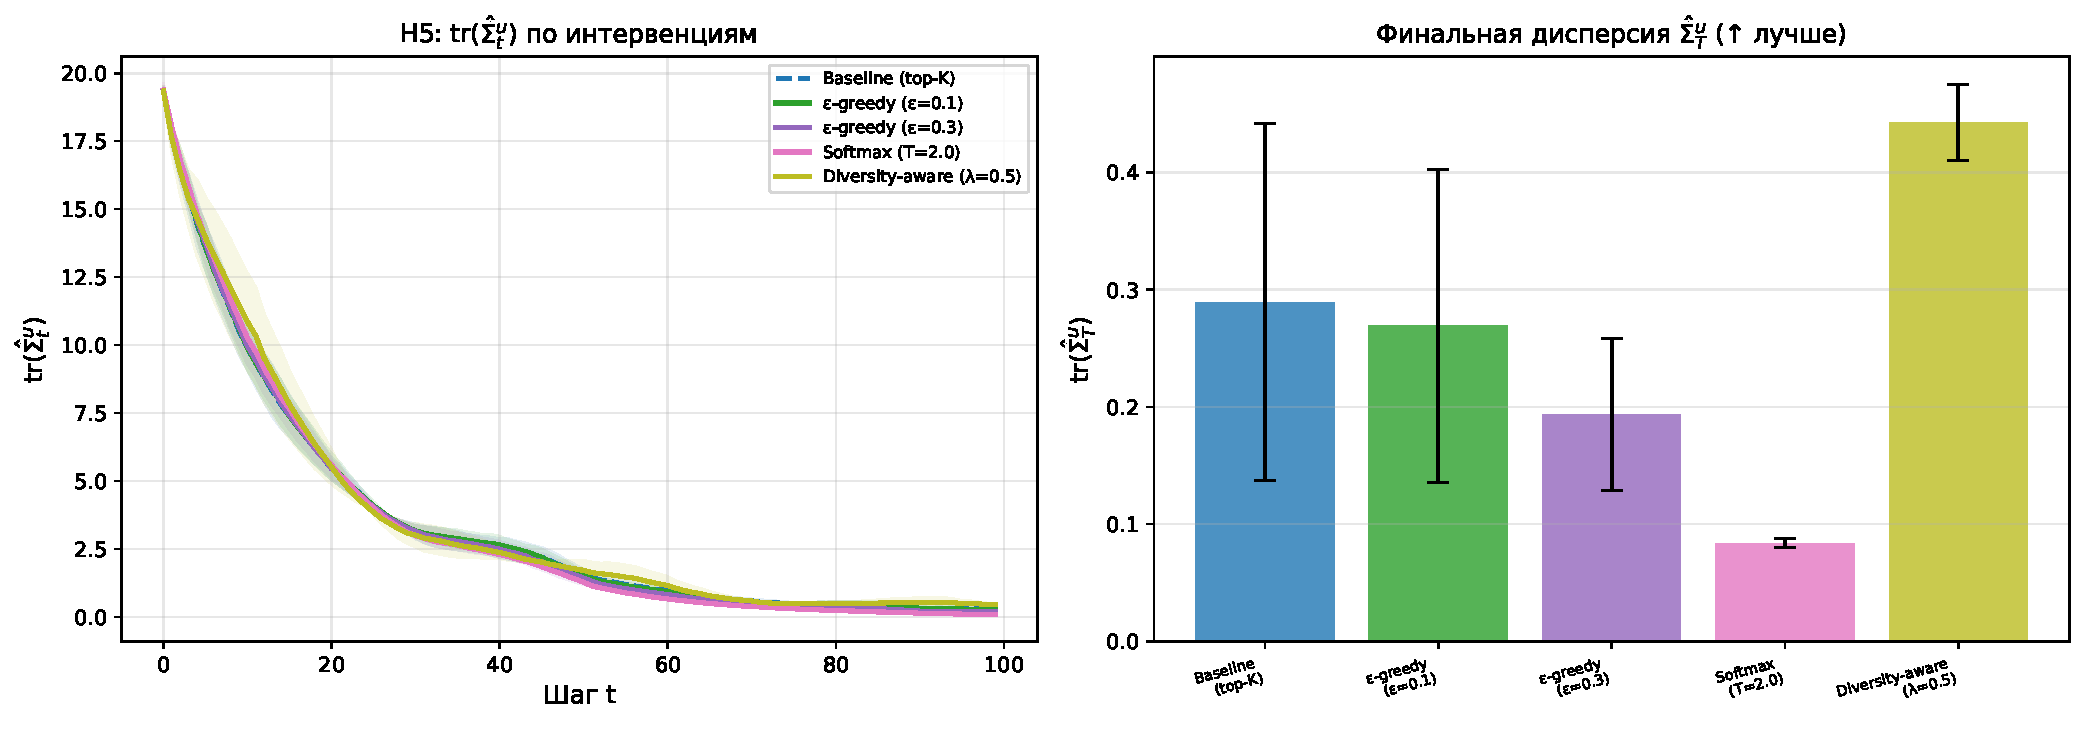
\includegraphics[width=\textwidth]{figures/H5_interventions_trace_sigma}
    \caption{Сохранение следа ковариации $\operatorname{tr}\hat\Sigma_t$ для пяти
    стратегий выдачи. Явный контроль разнообразия (MMR) сохраняет дисперсию выше
    базовой стратегии; случайные стратегии ($\varepsilon$-жадная, softmax)
    усиливают стягивание.}
    \label{fig:h5_trace}
\end{figure}

Результат содержит контринтуитивный вывод. Случайные стратегии~---
$\varepsilon$-жадная и softmax~--- стягивание не ослабляют, а \emph{усиливают}:
случайные показы выводят пользователей на объекты из разных сегментов, в среднем
расположенные ближе к центру пространства, и дрейф~\eqref{eq:drift} стягивает
всю популяцию к единой средней точке быстрее, чем жадная выдача. Напротив,
стратегия с явным контролем разнообразия сохраняет след ковариации
$0{,}442$ против $0{,}289$ у базовой~--- улучшение на $53\%$~--- при практически
том же качестве ($0{,}641$ против $0{,}634$). Механизм согласуется с
разделом~\ref{subsec:control_targets}: MMR штрафует за сходство показанных
объектов, поднимая $\sigma_\xi^2$, а значит и нижнюю грань разнообразия
Теоремы~\ref{thm:beta}. Компромисс качество--разнообразие для всех стратегий
показан на рис.~\ref{fig:h5_pareto}.

\begin{figure}[H]
    \centering
    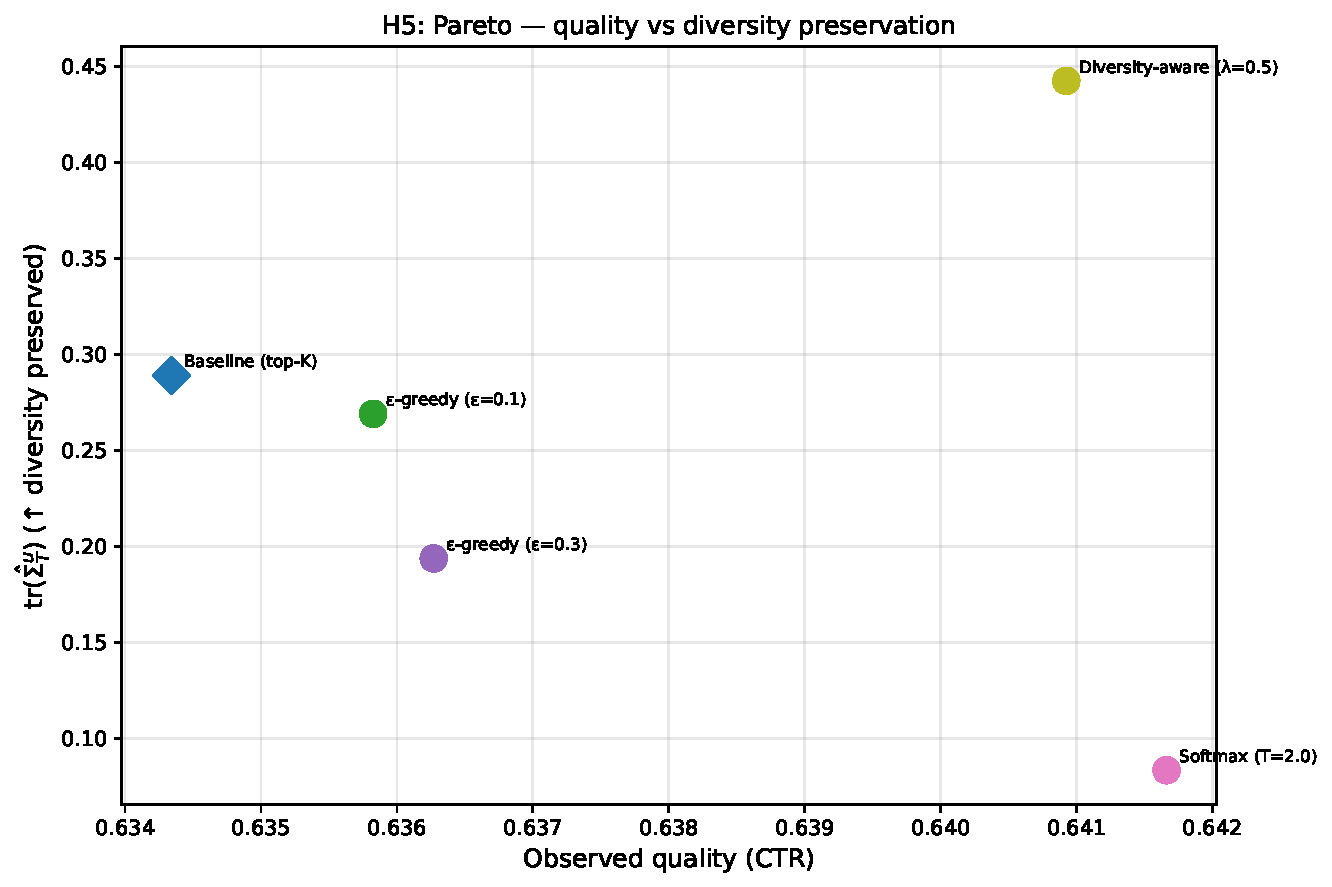
\includegraphics[width=0.8\textwidth]{figures/H5_pareto_quality_diversity}
    \caption{Компромисс между качеством выдачи и сохранением разнообразия для
    пяти стратегий. Стратегия с контролем разнообразия доминирует базовую,
    одновременно сохраняя качество.}
    \label{fig:h5_pareto}
\end{figure}

\textbf{Итог главы.} Управление контуром эффективно тогда, когда оно нацелено на
\emph{форму} выдачи, а не на её случайность. Случайное исследование не защищает
от стягивания и даже ускоряет его; защищает явное расширение выдачи в сочетании
с понижением загрязнения логов $\alpha=ps$. Тем самым на четвёртую задачу
раздела~\ref{subsec:questions} получен конструктивный ответ: предложен критерий
риска (таблица~\ref{tab:checklist}) и подтверждена работоспособность диверсификации
выдачи как меры подавления петлевого канала. В отличие от чисто эвристического
исследования выдачи, такой подход ближе к оптимальному управлению с ограничениями:
качество выдачи
должно оставаться не хуже приемлемого базового уровня, а управляющее воздействие
должно ограничивать накопление долгосрочного риска~\cite{chow2014baselineControl,
mariano2026optimalControl}.
 %% Управление петлёй обратной связи
    \newpage
    \section{Заключение}
\label{sec:Chapter6} \index{Chapter6}

Целью работы было построить математическую модель рекомендательного контура с
переобучением на собственных логах и установить условия его деградации, отделив
вклад переобучения от прочих причин. Вклад работы находится на стыке петель
обратной связи в рекомендательных системах, перформативного предсказания и
теории управления рекомендательными системами~\cite{krauth2022, perdomo2020,
depasquale2026controlSystems}. Поставленные задачи решены полностью.

\textbf{Задача~1.} Рекомендательная система формализована как замкнутая
стохастическая система управления (главы~\ref{sec:Chapter1}
и~\ref{sec:Chapter2}): определены состояние, управляющее воздействие, измерение,
функция перехода~\eqref{eq:closed_loop_transition} и закон адаптации регулятора;
выведено загрязнение логов~\eqref{eq:contaminated} и показано
(предложение~\ref{prop:self_reinforcement}), что обучение на загрязнённых логах
завышает наблюдаемые метрики относительно истинных~--- рост наблюдаемого качества
не равнозначен росту пользы. Этот вывод согласуется с работами о логированных
откликах, алгоритмическом смешении и каузальной коррекции данных
~\cite{sinha2016, chaney2018, bottou2013}.

\textbf{Задача~2.} Доказана Теорема~\ref{thm:beta} о стягивании разнообразия:
внутрикластерный разброс убывает геометрически с множителем $q=1-\beta\rho(2-\beta)$
к асимптотической нижней грани $\beta\sigma_\xi^2/(2-\beta)$. Получены следствия о
времени достижения эхо-камеры и о зависимости границы стягивания от концентрации
выдачи.

\textbf{Задача~3.} Установлено, что стягивание разнообразия универсально по
режиму: оно определяется дрейфом предпочтений и наступает даже без переобучения
(следствия~\ref{cor:no_beta} и~\ref{cor:universal}). Отдельно доказана
Теорема~\ref{thm:loop}: переобучение сужает ковариацию выдачи по сравнению с
замороженной моделью, опуская нижнюю грань разнообразия и переформировывая
ковариацию предпочтений. Тем самым переобучение оставляет отделимый след,
измеримый в дисперсионной части расхождения $\mathrm{KL}(P_T\Vert P_0)$; получены
условия его активации~--- различимость пользователей, наличие сегментной
структуры и порог концентрации.

\textbf{Задача~4.} Предсказания обеих теорем подтверждены серией вычислительных
экспериментов (глава~\ref{sec:Chapter4}), в том числе на наборе
\texttt{MovieLens-20M}: универсальность стягивания, отсутствие эффекта при
$\beta=0$, монотонность по $\alpha\rho$, локализация следа петли в дисперсии и
условие $K\ge2$. Предложен критерий риска и показано (глава~\ref{sec:Chapter5}),
что явная диверсификация выдачи сохраняет разнообразие лучше базовой стратегии
($+53\%$ при том же качестве), тогда как случайное исследование стягивание
усиливает.

Все полученные теоретические результаты строго доказаны и согласуются с
вычислительными экспериментами; центральный тезис работы~--- петля переобучения
оставляет специфический, отделимый от универсального дрейфа след в геометрии
ковариации предпочтений~--- установлен теоретически и подтверждён численно. В
терминах существующей литературы результат уточняет, какой именно компонент
обучения в замкнутом контуре отвечает за наблюдаемую деградацию: динамика с
состоянием даёт универсальное стягивание, а повторное переобучение меняет форму выдачи
~\cite{brown2022stateful, hardt2025performativePastFuture,
barlacchi2026diversityParadox}.

\textbf{Направления дальнейшей работы.} В построенной модели закон отклика
$\theta$ фиксирован, но его текущее значение $\theta_t^{ij}$ меняется вместе с
состоянием пользователя $u_i^t$. Естественным развитием является учёт автономной
динамики предпочтений, не сводящейся к воздействию потреблённых рекомендаций, а
также перенос теоретических оценок с фиксированной когорты на систему с уходом и
приходом пользователей. Перспективны прямое извлечение меры различимости пользователей
$\lVert J_k\rVert$ и резкости выдачи из весов обученной модели как эксплуатационных
метрик риска, раздельный анализ долей следования $s$ и использования $p$, а также
интервенции, нацеленные на форму ковариации выдачи. Отдельного внимания требует
каузальная оценка силы дрейфа $\beta$: полученная в
разделе~\ref{subsec:exp_real} граница по наблюдательным данным не отделяет
рекомендательно-индуцированный дрейф от автономной эволюции вкусов, и для такого
разделения необходима экзогенная вариация показов~--- рандомизованные показы
или регрессия на разрыве у границы отсечения списка. Практическая значимость
результатов состоит в том, что полученные условия допускают мониторинг по
наблюдаемым статистикам и могут служить основой раннего обнаружения деградации
персонализации в промышленных рекомендательных сервисах. Это направление
естественно продолжает каузальные методы для петель обратной связи и безопасные
постановки управления с ограничением на качество базовой политики
~\cite{krauth2022, chow2014baselineControl, chandrasekaran2026networkAware}.
 %% Заключение
    \newpage

    %% НЕ ТРОГАЙТЕ!!!
    \nocite{*}
    \bibliography{references}

    %% в зависимости от надобности подключаем раздел "Приложение"
    % \newpage
    % \input{Appendix.tex}
\end{document}
